% This is the Reed College LaTeX thesis template. Most of the work
% for the document class was done by Sam Noble (SN), as well as this
% template. Later comments etc. by Ben Salzberg (BTS). Additional
% restructuring and APA support by Jess Youngberg (JY).
% Your comments and suggestions are more than welcome; please email
% them to cus@reed.edu
%
% See http://web.reed.edu/cis/help/latex.html for help. There are a
% great bunch of help pages there, with notes on
% getting started, bibtex, etc. Go there and read it if you're not
% already familiar with LaTeX.
%
% Any line that starts with a percent symbol is a comment.
% They won't show up in the document, and are useful for notes
% to yourself and explaining commands.
% Commenting also removes a line from the document;
% very handy for troubleshooting problems. -BTS

% As far as I know, this follows the requirements laid out in
% the 2002-2003 Senior Handbook. Ask a librarian to check the
% document before binding. -SN

%%
%% Preamble
%%
% \documentclass{<something>} must begin each LaTeX document
\documentclass[12pt,twoside]{ugathesis}
% Packages are extensions to the basic LaTeX functions. Whatever you
% want to typeset, there is probably a package out there for it.
% Chemistry (chemtex), screenplays, you name it.
% Check out CTAN to see: http://www.ctan.org/
%%
\usepackage{graphicx,latexsym}
\usepackage[french]{babel}
\usepackage{amsmath}
\usepackage{amssymb,amsthm}
\usepackage{xcolor}
\usepackage{eso-pic}
\usepackage{longtable,booktabs,setspace}
\usepackage[hyphens]{url}
\usepackage{pdfpages}
\usepackage{tikz}
\usetikzlibrary{calc}
% Added by CII
\usepackage{hyperref}
\usepackage{lmodern}
\usepackage{float}
\floatplacement{figure}{H}
% End of CII addition
\usepackage{rotating}

% Next line commented out by CII
%%% \usepackage{natbib}
% Comment out the natbib line above and uncomment the following two lines to use the new
% biblatex-chicago style, for Chicago A. Also make some changes at the end where the
% bibliography is included.
%\usepackage{biblatex-chicago}
%\bibliography{thesis}


% Added by CII (Thanks, Hadley!)
% Use ref for internal links
\renewcommand{\hyperref}[2][???]{\autoref{#1}}
\def\chapterautorefname{Chapter}
\def\sectionautorefname{Section}
\def\subsectionautorefname{Subsection}
% End of CII addition

% Added by CII
\usepackage{caption}
\captionsetup{width=5in}
% End of CII addition

% \usepackage{times} % other fonts are available like times, bookman, charter, palatino


% To pass between YAML and LaTeX the dollar signs are added by CII
\title{THÈSE}
\author{Keurcien LUU}
\lab{Techniques de l'Ingénierie Médicale et de la Complexité - Informatique,
Mathématiques et Applications de Grenoble (TIMC-IMAG)}
\date{31 octobre 2017}
\division{Mathematics and Natural Sciences}
\advisor{Michael BLUM}

%\institution{}
%\degree{}

%%% Remember to use the correct department!
\department{Ingénierie de la Santé, de la Cognition et Environnement (EDISCE)}
% if you're writing a thesis in an interdisciplinary major,
% uncomment the line below and change the text as appropriate.
% check the Senior Handbook if unsure.
%\thedivisionof{The Established Interdisciplinary Committee for}
% if you want the approval page to say "Approved for the Committee",
% uncomment the next line
%\approvedforthe{Committee}

% Added by CII
%%% Copied from knitr
%% maxwidth is the original width if it's less than linewidth
%% otherwise use linewidth (to make sure the graphics do not exceed the margin)
\makeatletter
\def\maxwidth{ %
  \ifdim\Gin@nat@width>\linewidth
    \linewidth
  \else
    \Gin@nat@width
  \fi
}
\makeatother

\renewcommand{\contentsname}{Table of Contents}
% End of CII addition

\setlength{\parskip}{0pt}

% Added by CII

\providecommand{\tightlist}{%
  \setlength{\itemsep}{0pt}\setlength{\parskip}{0pt}}

\Acknowledgements{
The preface pretty much says it all. \par  Second paragraph of abstract
starts here.
}

\Dedication{

}

\Preface{
blabla \par
}

\Abstract{
** Résumé ** \par  La nécessité de développer des outils d'analyse
exploratoire capables de traiter de larges volumes de données. **
Abstract **
}

% End of CII addition
%%
%% End Preamble
%%
%
\begin{document}

% Everything below added by CII
  \maketitle

\frontmatter % this stuff will be roman-numbered
\pagestyle{empty} % this removes page numbers from the frontmatter
  \begin{acknowledgements}
    The preface pretty much says it all. \par  Second paragraph of abstract
    starts here.
  \end{acknowledgements}
  \begin{preface}
    blabla \par
  \end{preface}
  \hypersetup{linkcolor=black}
  \setcounter{tocdepth}{2}
  \tableofcontents

  \listoftables

  \listoffigures
  \begin{abstract}
    ** Résumé ** \par  La nécessité de développer des outils d'analyse
    exploratoire capables de traiter de larges volumes de données. **
    Abstract **
  \end{abstract}

\mainmatter % here the regular arabic numbering starts
\pagestyle{fancyplain} % turns page numbering back on

\chapter{Introduction}\label{introduction}

\section{La génétique des
populations}\label{la-genetique-des-populations}

\subsection{L'évolution comme point de
départ}\label{levolution-comme-point-de-depart}

« La génétique est la science de l'hérédité. Elle est la clé de toute la
biologie, parce qu'elle explique les mécanismes qui sont responsables de
la reproduction des êtres vivants, du fonctionnement et de la
transmission du matériel héréditaire, des différences entre les
individus, de l'évolution biologique. »

Cette définition, donnée par Cavalli-Sforza et traduite ici de l'italien
par Françoise Brun (L. Cavalli-Sforza, 1994), restitue également les
motivations à l'origine de l'émergence du domaine de la génétique des
populations, à savoir l'étude de la variabilité interindividuelle d'un
point de vue évolutionniste. Pour John H. Gillespie, il s'agit de la «
discipline qui fait le lien entre la génétique et l'évolution »
(Gillespie, 2010) : « La génétique des populations s'intéresse à
l'évolution d'un point de vue génétique. Elle diffère de la biologie en
ce que ses idées les plus importantes ne sont pas expérimentales ou
observationnelles mais davantage théoriques. Il pourrait difficilement
en être autrement. Les objets d'étude sont principalement la fréquence
et la valeur sélective des génotypes dans les populations naturelles. »

Malgré cette caractérisation, les fondements de la génétique des
populations trouvent en réalité leurs origines bien avant la
formalisation en 1909 par Wilhelm Johannsen du concept de gène et donc
de génotype (Roll-Hansen, 2014), en témoignent les travaux de Charles
Darwin (1809-1882) et de Gregor Mendel (1822-1884). \emph{L'Origine des
espèces}, publié en 1859 et considéré encore à ce jour comme le texte
fondateur de la théorie de l'évolution (Darwin, 1980), énonce les
premiers principes de la sélection naturelle. Les travaux de Mendel,
figurent quant à eux parmi les premiers à se pencher sur les mécanismes
de l'hérédité d'un point de vue statistique, notamment via l'étude de
phénotypes en termes de proportions et de fréquences.

\section{À l'origine de la variabilité
génétique}\label{a-lorigine-de-la-variabilite-genetique}

\subsection{La théorie de l'évolution}\label{la-theorie-de-levolution}

En 1859, Darwin soutenait l'idée selon laquelle la principale force
évolutive serait la sélection naturelle (Darwin, 1980). « Je me propose
de passer brièvement en revue les progrès de l'opinion relativement à
l'origine des espèces. Jusque tout récemment, la plupart des
naturalistes croyaient que les espèces sont des productions immuables
créées séparément. De nombreux savants ont habilement soutenu cette
hypothèse. Quelques autres, au contraire, ont admis que les espèces
éprouvent des modifications et que les formes actuelles descendent de
formes préexistantes par voie de génération régulière. » C'est de cette
manière qu'en 1920, Edmond Barbier, dans sa notice relative à la
traduction française de \emph{L'Origine des espèces} (Darwin, 1980),
décide de présenter le contexte dans lequel il a été amené à effectuer
ce travail de traduction. Bien qu'elle fut globalement bien accueillie
par la communauté scientifique, sa théorie fut tout de même en proie à
de nombreuses critiques. L'une des principales critiques émises à son
encontre fut relative à la croyance de Darwin selon laquelle l'hérédité
\emph{par mélange} serait le principal mode de transmission des
caractères héréditaires (Gayon, 1992). Or, si sélection naturelle il y
a, la conservation et la transmission des caractères sélectionnés est
essentielle. Si bien qu'une hérédité \emph{par mélange} n'est pas
envisageable pour soutenir la thèse de la sélection naturelle, puisque
tout caractère transmis de cette façon se verrait altéré (ou dilué si
l'on souhaite conserver l'idée de mélange) à chaque génération et donc
éliminé après un certain temps. Cependant, sa théorie bénéficiera par la
suite des travaux de Mendel qui, lors de leur redécouverte en 1902
(Bateson \& Mendel, 1913), apporteront l'élément fondamental manquant à
la théorie darwinienne : le principe d'hérédité \emph{mendélienne}.
Cette théorie de l'évolution néo-darwinienne, née de la conciliation de
la théorie darwinienne et du principe d'hérédité de Mendel, constitue le
paradigme évolutionniste tel que nous le connaissons aujourd'hui et
porte le nom de \emph{théorie synthétique de l'évolution}.

\subsection{L'évolution d'une théorie}\label{levolution-dune-theorie}

À la théorie néo-darwinienne est souvent opposée la théorie neutraliste
développée par Motoo Kimura dans son ouvrage \emph{The neutral theory of
molecular evolution} (Kimura, 1983), bien que ces deux théories ne
soient pas incompatibles. La première suggère que les mutations
apparaissent à la faveur de la sélection naturelle. La seconde affirme
quant à elle que l'évolution ne serait que le résultat de mutations qui
surviennent de façon tout à fait aléatoire, tout en étant sélectionnées
selon le même mécanisme de sélection naturelle proposé par Darwin.





\begin{figure}

{\centering \includegraphics{thesis_files/figure-latex/kimuravsdarwin-1} 

}

\caption{Représentation schématique des probabilités
d'occurrence pour chaque type de mutation pour la théorie sélectionniste
de Darwin et pour la théorie neutraliste de Kimura (Bromham \& Penny,
2003).}\label{fig:kimuravsdarwin}
\end{figure}
Une des composantes principales de cette nouvelle théorie consiste à
affirmer que les fluctuations aléatoires dans la fréquence des allèles,
n'affectant que très peu ou pas du tout la valeur sélective, constituent
la principale source de variabilité de l'ADN (B. Charlesworth \&
Charlesworth, 2009). Une grande partie de la variation génétique
observée est fonctionnellement neutre, n'occasionnant pas de changement
de phénotype.

\subsection{Sélection naturelle}\label{selection-naturelle}

\subsection{Sélection sexuelle}\label{selection-sexuelle}

\subsection{Dérive génétique}\label{derive-genetique}

La dérive génétique est un mécanisme important en génétique des
populations. Les modèles statistiques Nous illustrons ici le principe de
dérive génétique à l'aide du modèle de Wright-Fisher tel qu'il est
présenté dans l'ouvrage \emph{Population Genetics} (Gillespie, 2010).

Ten simulations of random genetic drift of a single given allele with an
initial frequency distribution 0.5 measured over the course of 50
generations, repeated in three reproductively synchronous populations of
different sizes. In these simulations, alleles drift to loss or fixation
(frequency of 0.0 or 1.0) only in the smallest population





\begin{figure}

{\centering 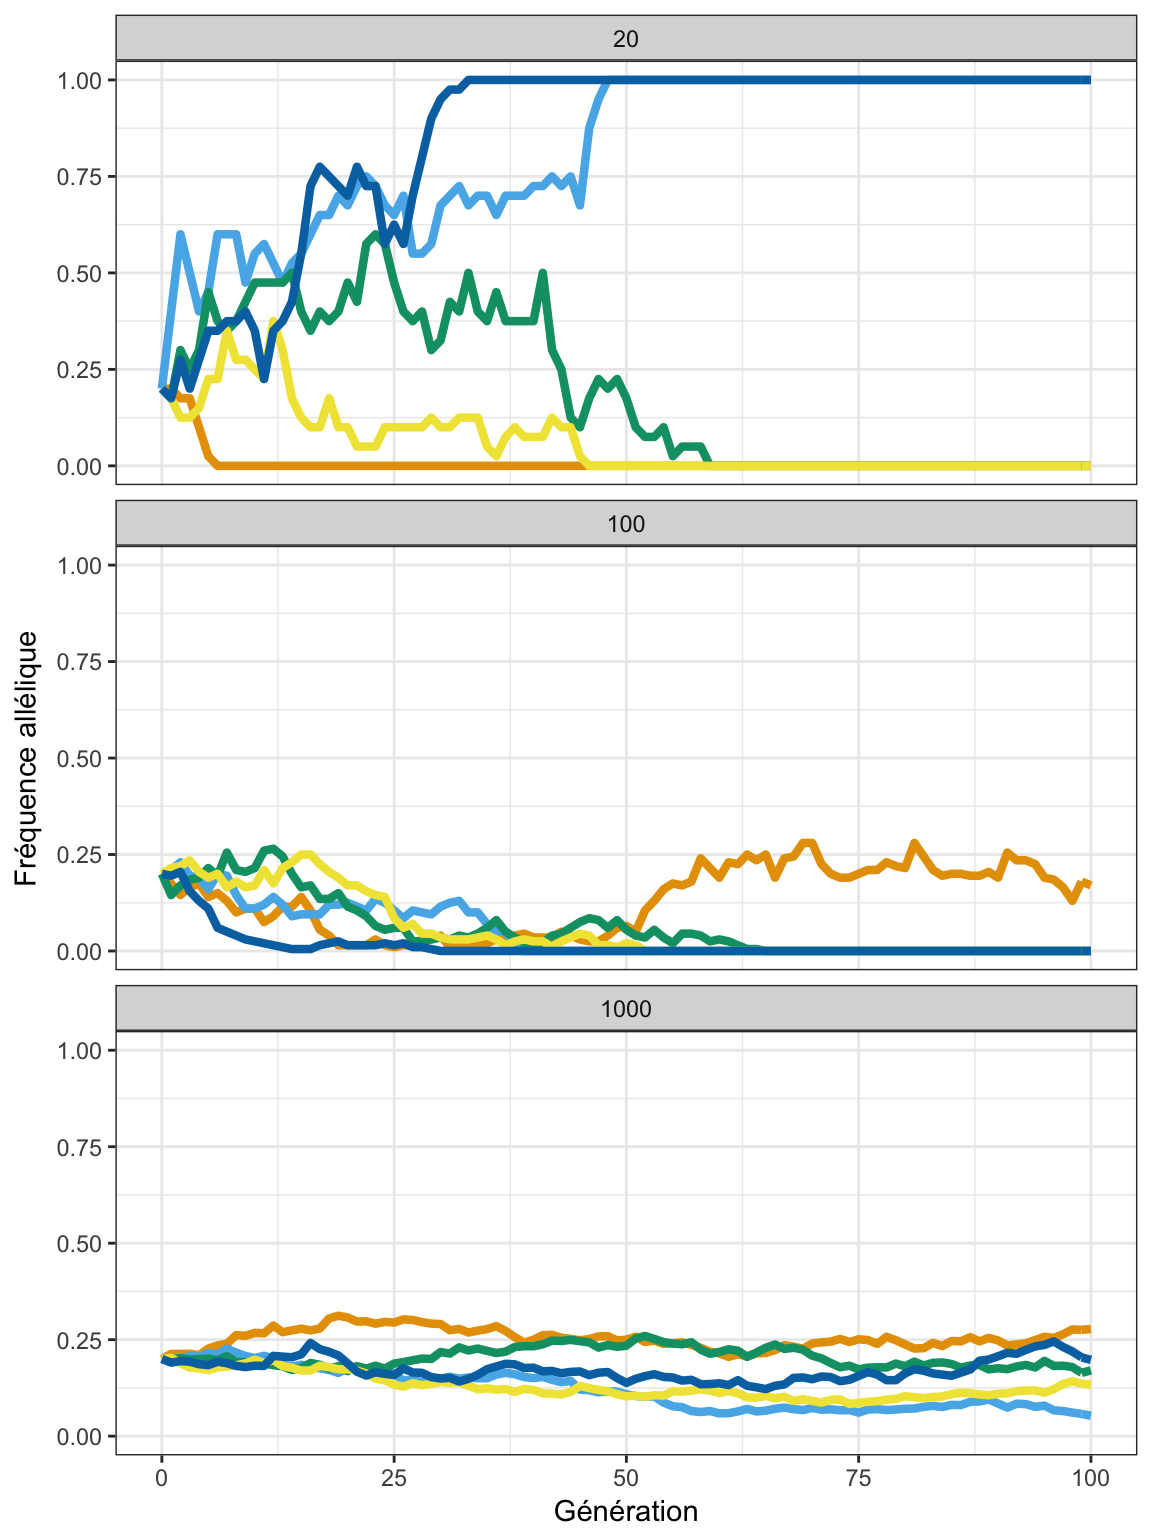
\includegraphics{thesis_files/figure-latex/drift-1} 

}

\caption{Simulation numérique de la dérive génétique. La
fréquence de l'allèle étudié est simulée pour 5 populations constituées
chacune de 20 individus sur une période de 100 générations. Dans chaque
population, la fréquence de l'allèle est initialement de 0.20.}\label{fig:drift}
\end{figure}
La fréquence d'un allèle au sein d'une population est principalement
impactée par deux facteurs :
\begin{itemize}
\item
  Le nombre d'individus composant la population
\item
  Les lois de Mendel
\end{itemize}
La figure \ref{fig:drift} met en évidence deux propriétés de la dérive
génétique :
\begin{itemize}
\item
  Les fréquences alléliques évoluent de façon indépendante d'une
  population à une autre.
\item
  La dérive génétique entraîne une perte de diversité allélique au sein
  des populations de petite taille. Dans le modèle de Wright-Fisher, les
  fréquences alléliques finissent éventuellement par atteindre les états
  dits absorbants que sont \(0\) et \(1\).
\end{itemize}
Wiki : ``En particulier, l'hypothèse de neutralité, sous laquelle les
mutations n'ont aucune influence sur la valeur sélective, est
l'hypothèse nulle généralement retenue dans les travaux où une telle
hypothèse est nécessaire.''

La formulation d'une hypothèse ou d'un ensemble d'hypothèses permettant
de décrire un processus évolutif en l'absence de sélection, portant
généralement le nom de \emph{modèle neutre}, est souvent de première
nécessité dans toute démarche visant à caractériser un mécanisme de
sélection. La donnée d'observations mettant en défaut le modèle neutre
aura pour conséquences de créditer davantage une hypothèse invoquant un
processus de sélection.

\subsection{Mutations aléatoires}\label{mutations-aleatoires}

Si la dérive génétique entraîne une perte de diversité allélique, les
mutations favorisent quant à elle le maintien des variations génétiques
entre les populations (Gillespie, 2010). Une mutation peut survenir à un
locus donné avec une probabilité spécifique à chaque espèce, appelée
\emph{taux de mutation}.

\subsection{Flux de gène}\label{flux-de-gene}

Le flux de gène est le résultat d'évènements migratoires, initiés par
des individus appartenant à une population donnée, vers une seconde
population dont le pool génique diffère éventuellement de la population
d'origine.
\begin{center}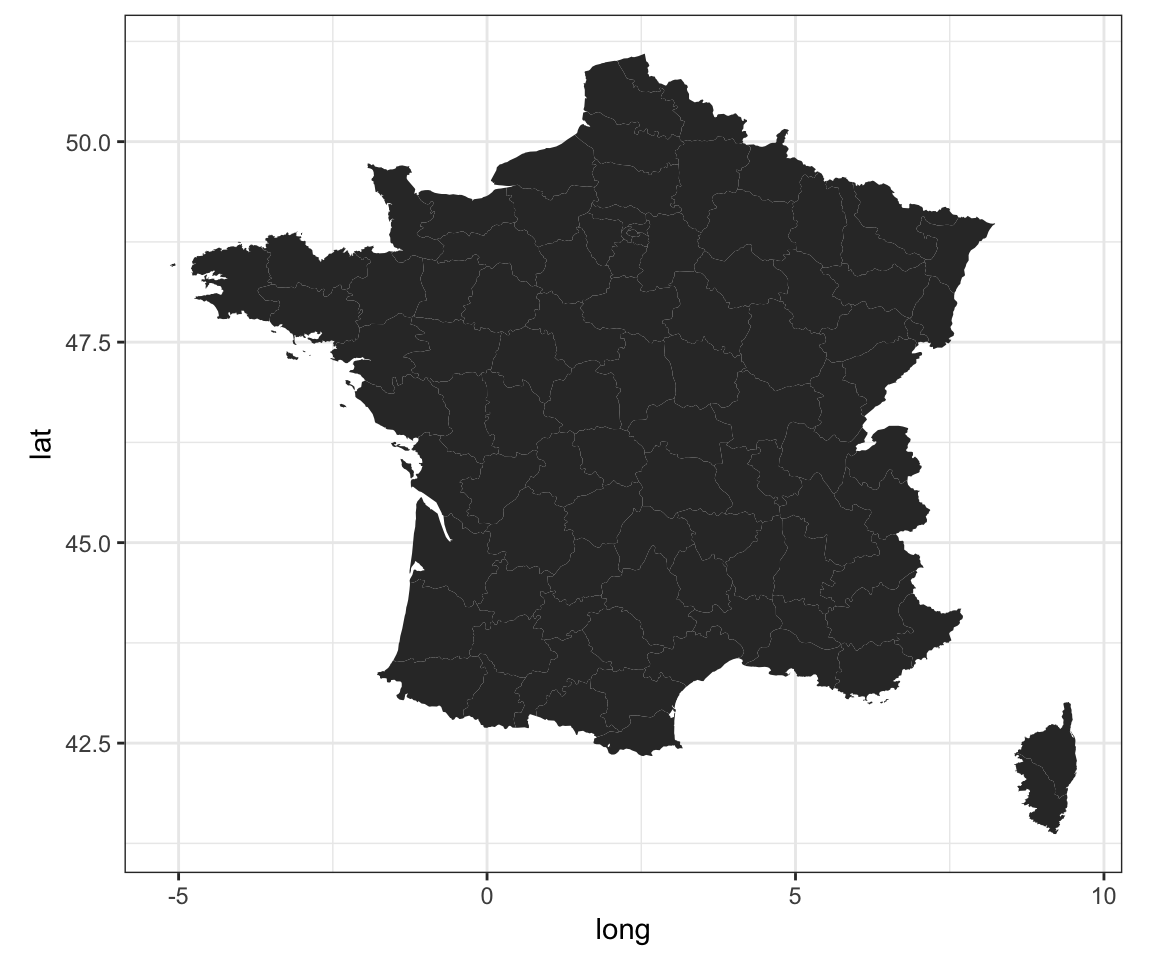
\includegraphics{thesis_files/figure-latex/unnamed-chunk-1-1} \end{center}

\section{Adaptation}\label{adaptation}

\subsection{Adaptation locale}\label{adaptation-locale}

Haut plateau, Lactase (Jeong \& Di Rienzo, 2014)

Sélection naturelle Environnement hétérogène

\section{Données de séquençage nouvelle
génération}\label{donnees-de-sequencage-nouvelle-generation}

\subsection{Next-Generation Sequencing
(NGS)}\label{next-generation-sequencing-ngs}

Exome, Genome, transcriptome, etc\ldots{}

Le séquençage nouvelle génération a connu un essor considérable au cours
des dernières décennies. Si bien que les prouesses techniques et les
progrès technologiques réalisés dans ce domaine ont permis de réduire
d'un facteur 100,000 les coûts de séquençage en l'espace de seulement 15
ans (Wetterstrand, 2013).



\begin{figure}

{\centering 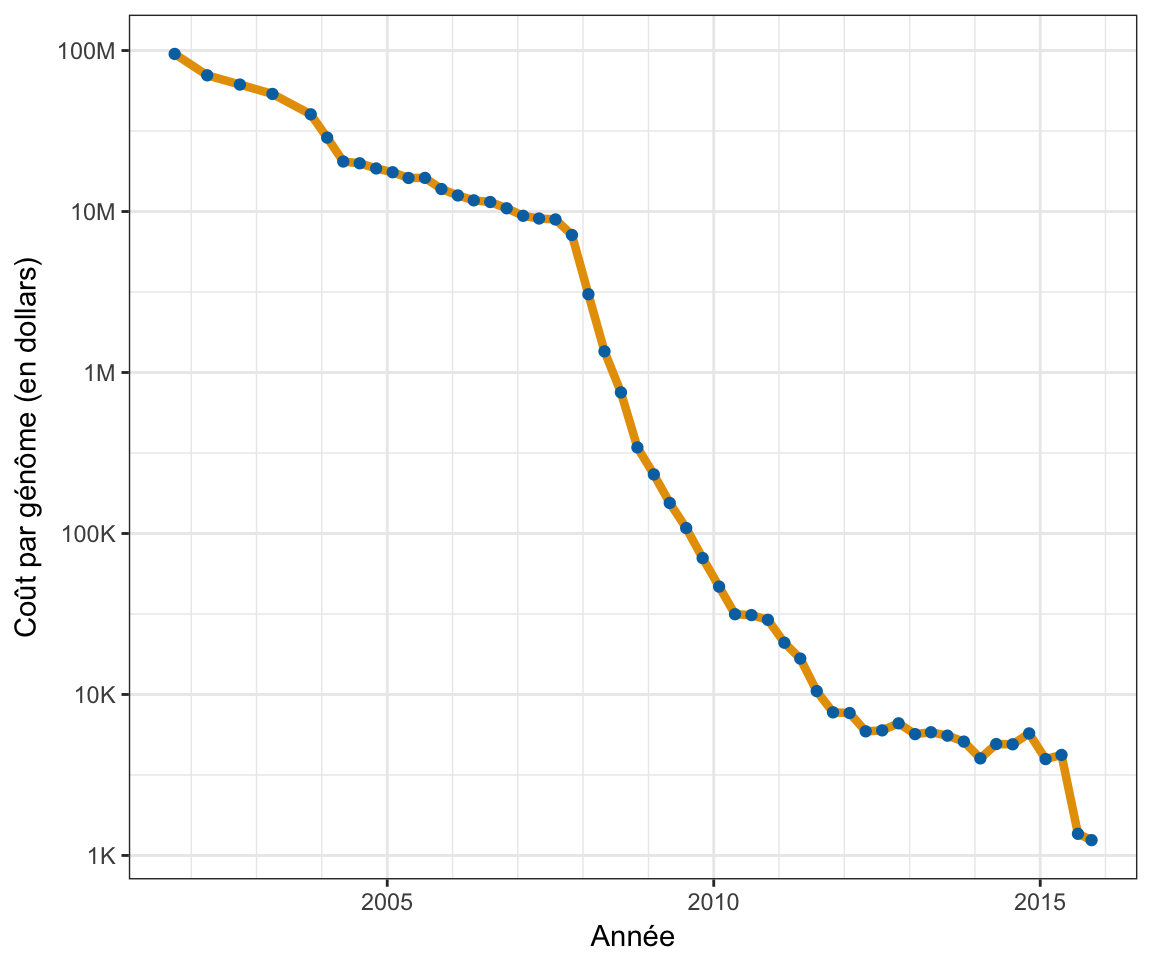
\includegraphics{thesis_files/figure-latex/wetterstrand-1} 

}

\caption{Évolution des coûts de séquençage depuis 2001
(Wetterstrand, 2013).}\label{fig:wetterstrand}
\end{figure}
Le séquençage nouvelle génération génèrant de considérables volumes de
données, de nouvelles problèmatiques se posent quant à leur stockage et
leur analyse, nécessitant l'utilisation de puissantes ressources de
calcul ainsi que le développement d'algorithmes plus adaptés
(Gogol-Döring \& Chen, 2012). Financement croissant pour l'acquisition
de données NGS (Muir et al., 2016).

\subsection{}\label{section}

L'accumulation de données, aussi bien en termes d'observations qu'en
termes de variables, laisse à penser que le traitement de celles-ci
pourrait permettre de détecter efficacement les variables qui sont
responsables ou qui influencent un phénomène particulier. Cela pourrait
être par exemple l'utilisation de bases de données automobiles pour
prédire la durée de vie de véhicules neufs, ou encore celle de données
climatiques pour estimer les variations de température auxquelles
pourrait être sujette notre planète. Cette accumulation massive
s'accompagne tout de même d'un phénomène bien connu en statistiques,
phénomène qui porte le nom de ``curse of dimensionality'' (Giraud,
2014).

\subsection{Les marqueurs génétiques}\label{les-marqueurs-genetiques}

Au concept de génétique est souvent associé l'acronyme ADN,
correspondant au nom de la molécule d'Acide désoxyribonucléique.

DNA bases pair up with each other, A with T and C with G, to form units
called base pairs. Each base is also attached to a sugar molecule and a
phosphate molecule. Together, a base, sugar, and phosphate are called a
nucleotide. Nucleotides are arranged in two long strands that form a
spiral called a double helix. The structure of the double helix is
somewhat like a ladder, with the base pairs forming the ladder's rungs
and the sugar and phosphate molecules forming the vertical sidepieces of
the ladder. \url{https://ghr.nlm.nih.gov/primer/basics/dna} Chaque
chromosome est constitué de deux brins d'ADN. La structure spatiale de
l'ADN n'étant pas prise en compte dans les travaux présentés ici, nous
en garderons une représentation unidimensionnelle.

D'un point de vue statistique, seuls les sites nucléotidiques
potentiellement variables d'une observation à une autre présentent un
intérêt. Ces variations génétiques peuvent se manifester sous
différentes formes, nous amenant à les classer d'autant de façons :
\begin{itemize}
\tightlist
\item
  Microsatellite :
\end{itemize}
Jusqu'à présent, les microsatellites ont connu un succès important,
notamment grâce à la popularisation de techniques telles que la PCR
(\emph{Polymerase Chain Reaction}). Leur étude a permis de mettre en
évidence l'implication de divers blablabla. Un microsatellite est
repérable par la répétition successive de petits motifs chacun composé
de 1 à 4 acides aminés.




\begin{figure}

{\centering 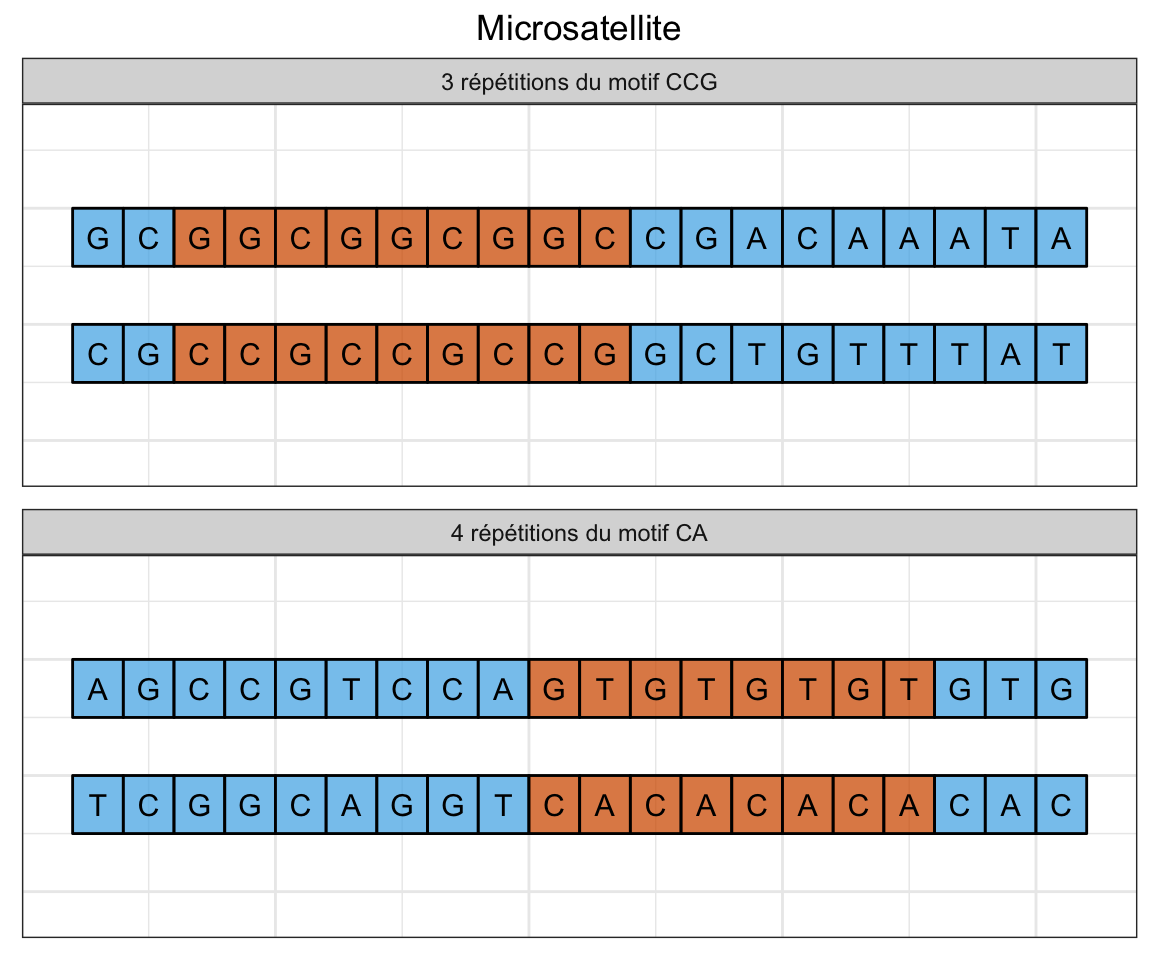
\includegraphics{thesis_files/figure-latex/microsat-1} 

}

\caption{Exemples de microsatellites. La première séquence
comporte 3 répétitions du motif CCG, tandis que la seconde inclut 4
répétitions du motif CA.}\label{fig:microsat}
\end{figure}
\begin{itemize}
\tightlist
\item
  Indel :
\end{itemize}
INDEL (INsertion/DELetion) is where a single base has been deleted, or
inserted into one genome relative to another. It is a symmetrical
relationship, as a deletion in one corresponds to an insertion in
another.
\begin{center}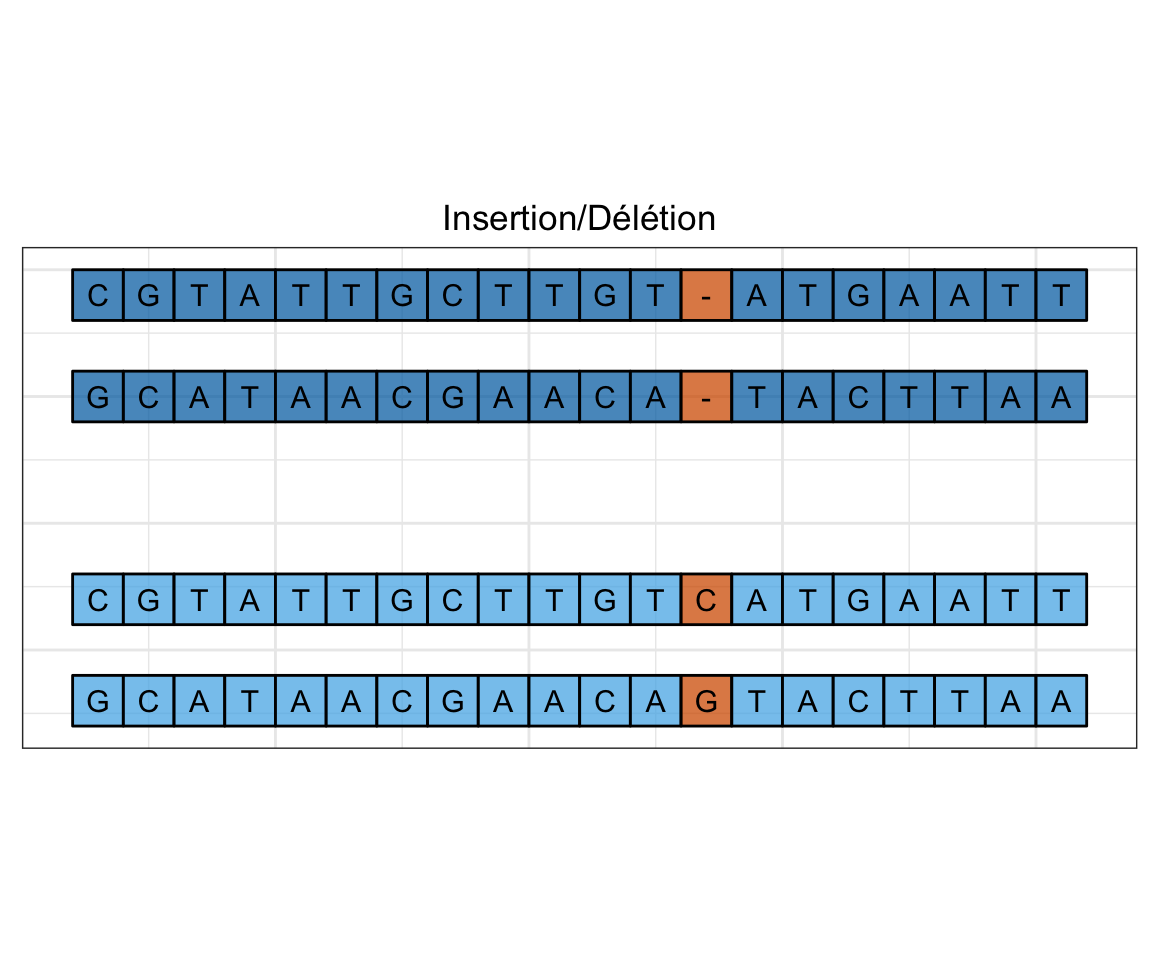
\includegraphics{thesis_files/figure-latex/indel-1} \end{center}
\begin{itemize}
\tightlist
\item
  Polymorphisme nucléotidique :
\end{itemize}
\begin{center}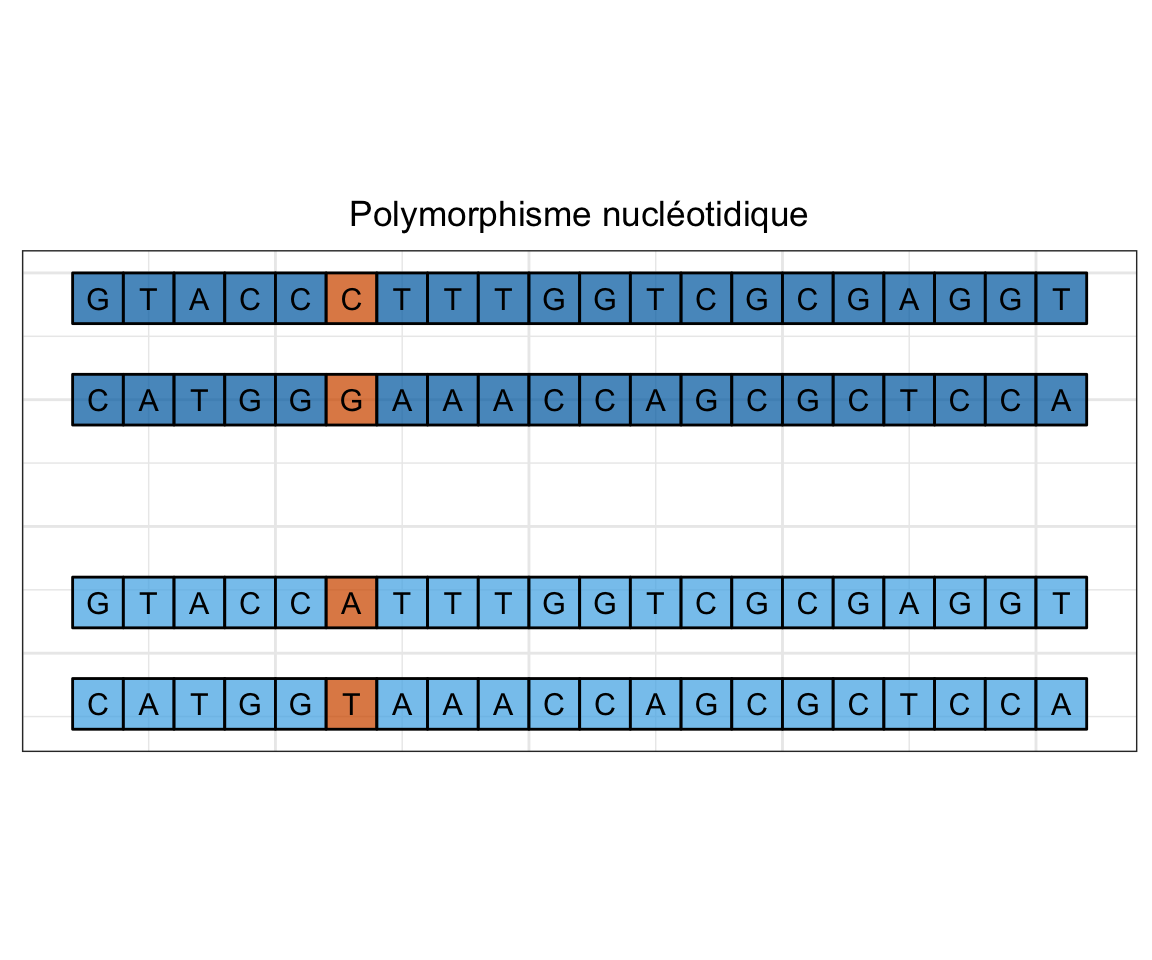
\includegraphics{thesis_files/figure-latex/snp-1} \end{center}

\chapter{État de l'art}\label{etat-de-lart}

\section{L'indice de fixation}\label{lindice-de-fixation}

En se différenciant génétiquement, les populations voient leurs
fréquences d'allèles évoluer de façon indépendante. L'indice de fixation
est une statistique permettant de quantifier pour un allèle donné,
l'écart de la fréquence observée dans une sous-population à la fréquence
théorique

\section{Modèle de FLK}\label{modele-de-flk}

Le modèle de FLK estime le modèle neutre d'un SNP bi-allélique lorsque
celui-ci est uniquement soumis à la dérive génétique. À l'instant
\(t = 0\), le SNP a une fréquence \(p_0\). Notant \(F_t\) l'indice de
fixation de cet allèle, \(p(t)\) sa fréquence après \(t\) générations,
et en supposant que \(F_t\) soit suffisamment petit, ce qui devrait être
vérifié dans le cas neutre. (Nicholson et al., 2002) :
\begin{equation} 
  p(t) \sim N(p_0, F_t p_0 (1-p_0)) 
  \label{eq:frequency-law}
\end{equation}
De la loi \eqref{eq:frequency-law} nous tirons
\(\text{Var}(p(t)) = F_t p_0 (1-p_0)\).

La statistique FLK (Bonhomme et al., 2010) requiert d'estimer au
préalable deux paramètres que sont la fréquence allélique initiale
\(p_0\) et la matrice d'apparentement \(V\), \(V \in M_K(\mathbb{R})\)
où \(K\) est le nombre de populations observées. Notant :
\begin{itemize}
\item
  \(\boldsymbol{p} = (p_1, p_2, \dots, p_K) \in \mathbb{R}^K\),
\item
  \(\boldsymbol{p_0} = (p_0, p_0, \dots, p_0) \in \mathbb{R}^K\),
\item
  \(\boldsymbol{r} = N(0, V)\),
\end{itemize}
le modèle neutre pour \(\boldsymbol{p}\) est donné par la relation
suivante :
\begin{equation} 
  \boldsymbol{p} = \boldsymbol{p_0} + \boldsymbol{r} 
  \label{eq:flk_neutral_model}
\end{equation}
Bonhomme \textit{et al.} proposent pour ce modèle de mesurer une
statistique de qualité de l'ajustement pour quantifier la déviance d'un
allèle par rapport au modèle neutre :
\begin{equation} 
  FLK = (\boldsymbol{p - \hat{p}_0})^T V (\boldsymbol{p - \hat{p}_0})                                \label{eq:flk-statistic}
\end{equation}
Sous l'hypothèse neutre et suivant \eqref{eq:flk-statistic},
\(FLK \sim \chi^2 (K - 1)\).

\section{Modèle de OutFLANK}\label{modele-de-outflank}

En reprenant le modèle proposé par Lewontin et Krakauer (Lewontin \&
Krakauer, 1973) et en y apportant les corrections nécessaires afin de
prendre en compte les erreurs d'échantillonnage, Whitlock
\textit{et al.} proposent une méthode permettant de détecter les allèles
sous sélection en environnement hétérogène (Whitlock \& Lotterhos,
2015). Ainsi, la quantité
\begin{equation} 
  k \frac{F_{ST}^{\prime}}{\bar{{F_{ST}^{\prime}}}}  
  \label{eq:OutFLANK-statistic}
\end{equation}
où \(k\) représente le nombre de degrés de libertés.

\section{Modèle du logiciel Bayescan}\label{modele-du-logiciel-bayescan}

Bayescan est aujourd'hui encore un des logiciels les plus utilisés pour
détecter l'adaptation locale. Le modèle employé suppose que les
sous-populations observées proviennent toutes d'une même population
ancestrale. Pour une sous-population donnée et un SNP donné, la
statistique de \(F_{ST}\) peut être estimée en utilisant la
vraisemblance d'un modèle multinomial-Dirichlet (Beaumont \& Balding,
2004). \(F_{ST} \in [0, 1]\) est une quantité qui peut être interprété
comme proportionnel à la probabilité que deux individus aient un ancêtre
commun dans la sous-population
\begin{equation} 
  \log \left( \frac{F_{ST}}{1 - F_{ST}} \right) = \alpha_j + \beta_i + \gamma_{ij}
  \label{eq:Bayescan-statistic}
\end{equation}
\section{Fast PCA}\label{fast-pca}

\subsection{L'ACP en génétique des
populations}\label{lacp-en-genetique-des-populations}

L'utilisation de l'Analyse en Composantes Principales en génétique des
populations a été popularisée par Cavalli-Sforza (Menozzi, Piazza, \&
Cavalli-Sforza, 1978).



\begin{figure}

{\centering 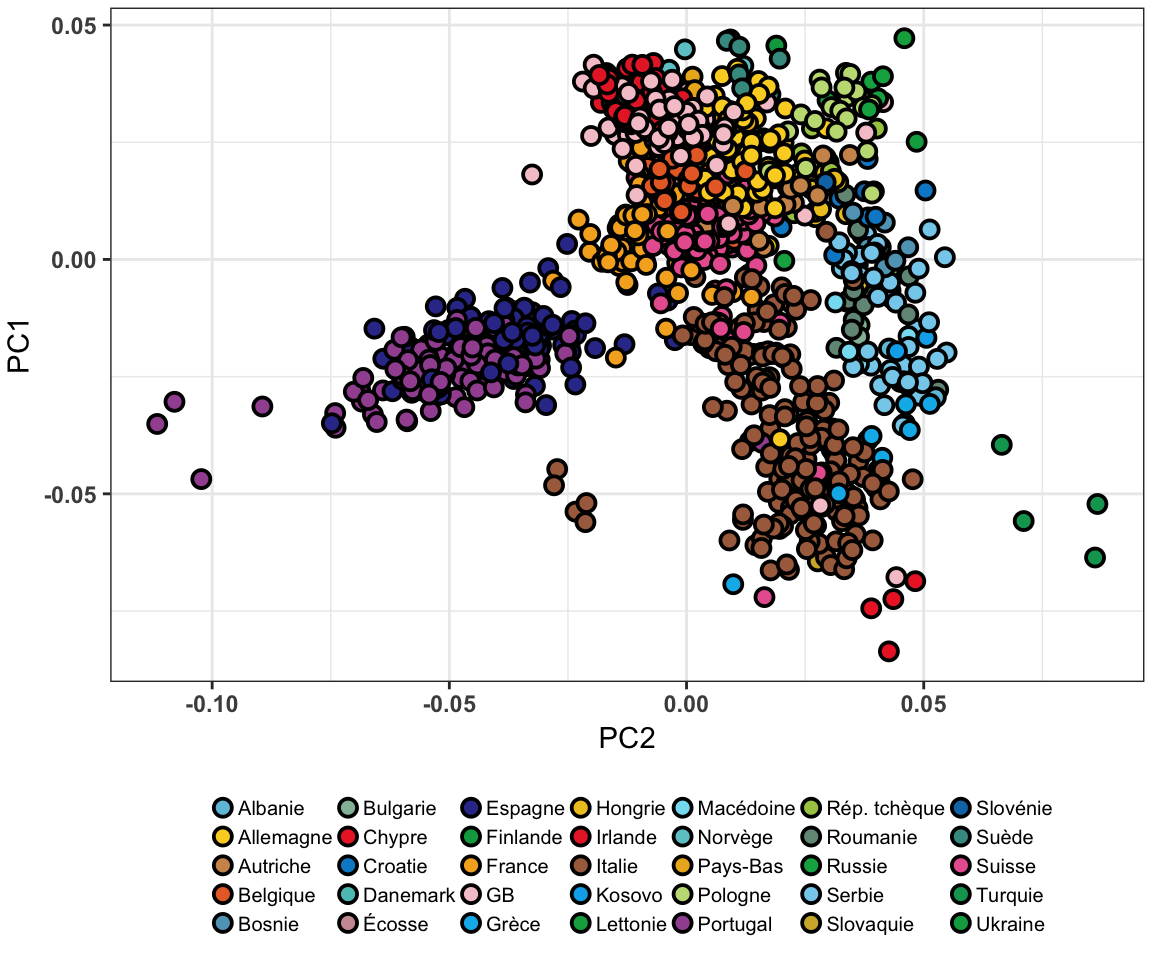
\includegraphics{thesis_files/figure-latex/popres-1} 

}

\caption{ACP réalisée sur le jeu de données POPRES (Novembre et
al., 2008).}\label{fig:popres}
\end{figure}
\section{Analyse en Composantes Principales
parcimonieuse}\label{analyse-en-composantes-principales-parcimonieuse}

\section{Bootstrap ACP}\label{bootstrap-acp}

\section{Contexte}\label{contexte}

\section{Tests multiples}\label{tests-multiples}

\section{Contrôle du taux de fausse
découverte}\label{controle-du-taux-de-fausse-decouverte}

Le taux de fausse découverte, correspond à la proportion de faux
positifs parmi les positifs. En notant \(FP\) le nombre de faux
positifs, \(FP\) le nombre de vrais positifs, on définit le taux de
fausse découverte \(FDR\) par :
\[ FDR = \mathbb{E}\Big[\frac{FP}{TP + FP} 1_{FP+TP > 0}\Big] \] -
Référence cours de Christophe Giraud

q-value, bonferroni, benjamini-hochberg La figure suivante donne les
comparaisons entre les différentes procédures de correction :

\chapter{Adaptation locale}\label{adaptation-locale-1}

Une population est dite localement adaptée à son environnement si elle a
connu une évolution différente de celles qu'ont connu les autres
populations de la même espèce, et ce, en réponse aux pressions
sélectives auxquelles elle peut être confrontrée.

\section{Cas d'étude utilisant
pcadapt}\label{cas-detude-utilisant-pcadapt}

\section{Simulations et modèles
démographiques}\label{simulations-et-modeles-demographiques}

\subsection{Modèle en île}\label{modele-en-ile}
\begin{center}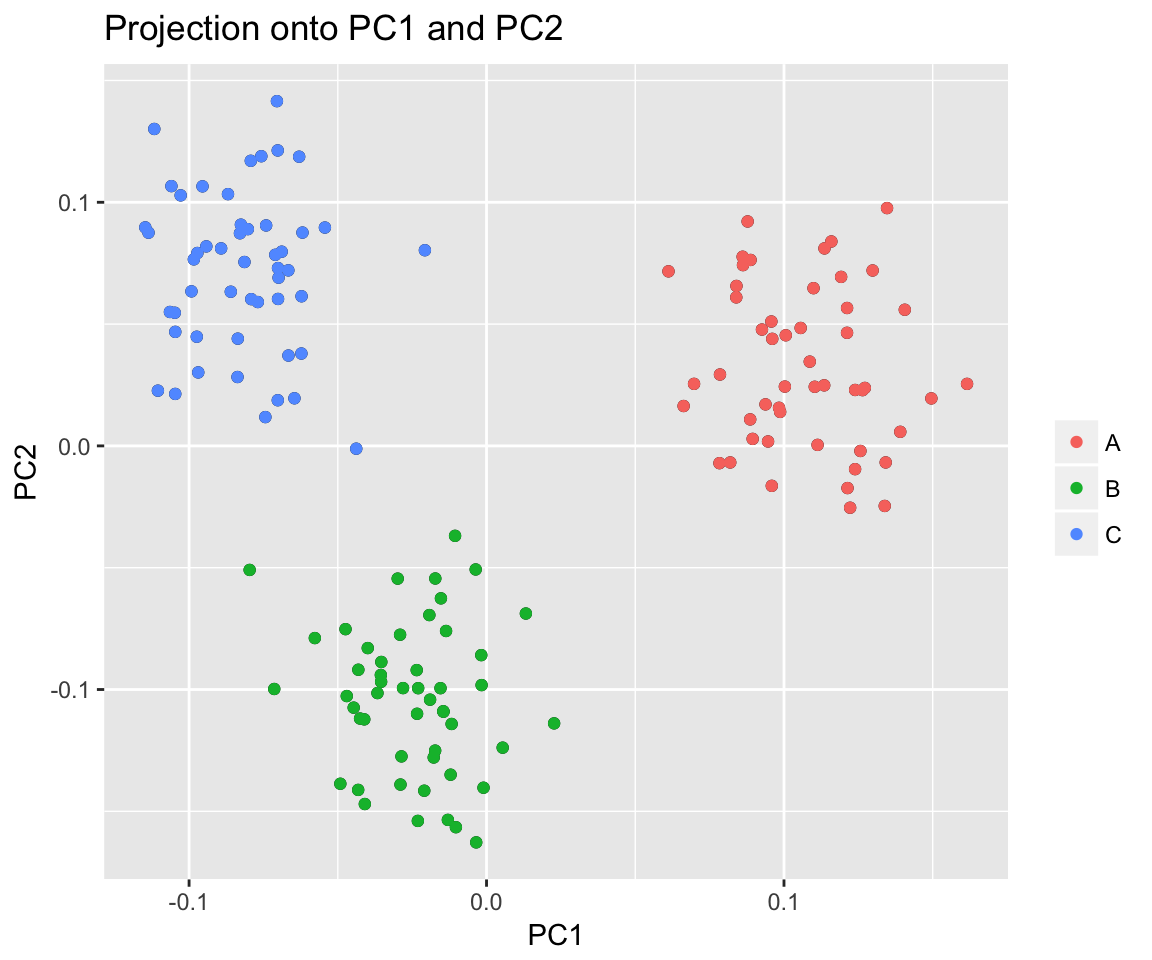
\includegraphics{thesis_files/figure-latex/island-pca-1} \end{center}
\begin{center}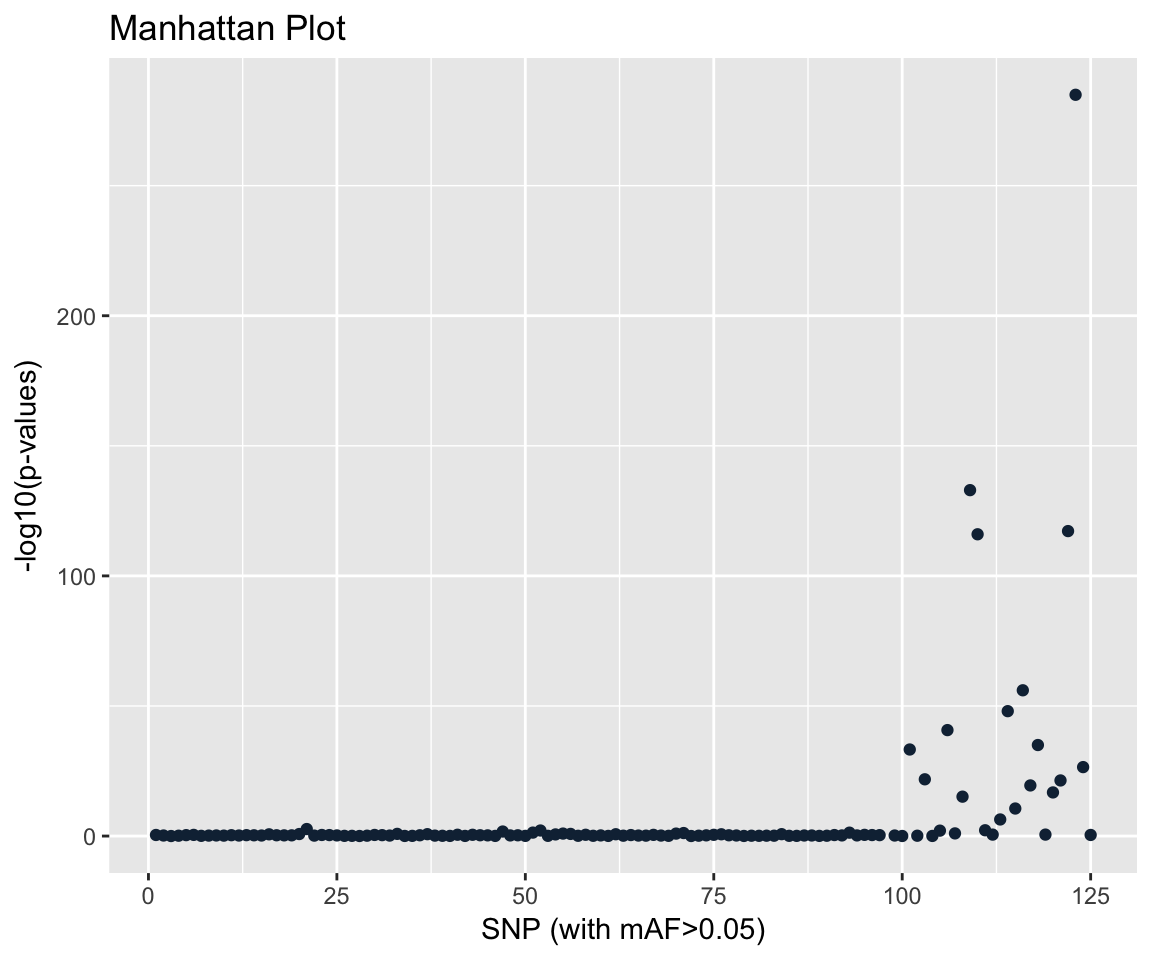
\includegraphics{thesis_files/figure-latex/island-manhattan-1} \end{center}

\subsection{Modèle de divergence}\label{modele-de-divergence}

Nous adaptons une version du script Python utilisé dans (Roux et al.,
2012), basé sur le module de simulation simuPOP (Peng \& Kimmel, 2005).
\begin{Shaded}
\begin{Highlighting}[]
\CommentTok{#!/usr/bin/env python}
\ImportTok{from} \NormalTok{__future__ }\ImportTok{import} \NormalTok{division}
\ImportTok{import} \NormalTok{simuOpt, types, os, sys, time}
\NormalTok{simuOpt.setOptions(alleleType }\OperatorTok{=} \StringTok{'long'}\NormalTok{)}
\ImportTok{from} \NormalTok{operator }\ImportTok{import} \NormalTok{itemgetter}
\ImportTok{import} \NormalTok{numpy }\ImportTok{as} \NormalTok{np}
\ImportTok{from} \NormalTok{simuPOP }\ImportTok{import} \OperatorTok{*}
\ImportTok{from} \NormalTok{simuPOP.utils }\ImportTok{import} \OperatorTok{*}
\ImportTok{from} \NormalTok{simuPOP.sampling }\ImportTok{import} \NormalTok{drawRandomSample}

\KeywordTok{def} \NormalTok{simulate(Ne, Nsam, T1, T2, T3, s10, s11):}
    \NormalTok{pop }\OperatorTok{=} \NormalTok{Population(size }\OperatorTok{=} \NormalTok{Ne, }
                     \NormalTok{ploidy }\OperatorTok{=} \DecValTok{2}\NormalTok{, }
                     \NormalTok{loci }\OperatorTok{=} \NormalTok{[}\DecValTok{1}\NormalTok{], }
                     \NormalTok{infoFields }\OperatorTok{=} \NormalTok{[}\StringTok{'fitness'}\NormalTok{, }\StringTok{'migrate_to'}\NormalTok{])}
                     
    \KeywordTok{def} \NormalTok{getfitness10(geno):}
        \ControlFlowTok{if} \NormalTok{geno[}\DecValTok{0}\NormalTok{] }\OperatorTok{+} \NormalTok{geno[}\DecValTok{1}\NormalTok{] }\OperatorTok{==} \DecValTok{0} \NormalTok{:}
            \ControlFlowTok{return} \DecValTok{1} \OperatorTok{-} \DecValTok{2} \OperatorTok{*} \NormalTok{s10}
        \ControlFlowTok{if} \NormalTok{geno[}\DecValTok{0}\NormalTok{] }\OperatorTok{+} \NormalTok{geno[}\DecValTok{1}\NormalTok{] }\OperatorTok{==} \DecValTok{1} \NormalTok{:}
            \ControlFlowTok{return} \DecValTok{1} \OperatorTok{-} \NormalTok{s10}
        \ControlFlowTok{else} \NormalTok{:}
            \ControlFlowTok{return} \DecValTok{1}

    \KeywordTok{def} \NormalTok{getfitness11(geno):}
        \ControlFlowTok{if} \NormalTok{geno[}\DecValTok{0}\NormalTok{] }\OperatorTok{+} \NormalTok{geno[}\DecValTok{1}\NormalTok{] }\OperatorTok{==} \DecValTok{0} \NormalTok{:}
            \ControlFlowTok{return} \DecValTok{1} \OperatorTok{-} \DecValTok{2} \OperatorTok{*} \NormalTok{s11}
        \ControlFlowTok{if} \NormalTok{geno[}\DecValTok{0}\NormalTok{] }\OperatorTok{+} \NormalTok{geno[}\DecValTok{1}\NormalTok{] }\OperatorTok{==} \DecValTok{1} \NormalTok{:}
            \ControlFlowTok{return} \DecValTok{1} \OperatorTok{-} \NormalTok{s11}
        \ControlFlowTok{else} \NormalTok{:}
            \ControlFlowTok{return} \DecValTok{1}
            
    \NormalTok{pop.evolve( }
        \NormalTok{initOps }\OperatorTok{=} \NormalTok{[}
            \NormalTok{InitSex(),}
            \NormalTok{InitGenotype(loci }\OperatorTok{=} \NormalTok{ALL_AVAIL, }
                         \NormalTok{freq }\OperatorTok{=} \NormalTok{[}\FloatTok{0.5}\NormalTok{, }\FloatTok{0.5}\NormalTok{],  }
                         \NormalTok{begin }\OperatorTok{=} \DecValTok{0}\NormalTok{, }
                         \NormalTok{end }\OperatorTok{=} \DecValTok{1}\NormalTok{)}
        \NormalTok{],}
        
        \NormalTok{preOps }\OperatorTok{=} \NormalTok{[}
            \CommentTok{# resize the ancestral population at the time immediatly }
            \CommentTok{# before the split}
            \NormalTok{ResizeSubPops([}\DecValTok{0}\NormalTok{], }
                          \NormalTok{sizes }\OperatorTok{=} \NormalTok{[Ne }\OperatorTok{+} \NormalTok{Ne], }
                          \NormalTok{at }\OperatorTok{=} \NormalTok{T1 }\OperatorTok{-} \DecValTok{1}\NormalTok{),}
                              
            \NormalTok{ResizeSubPops([}\StringTok{"S1_1"}\NormalTok{], }
                          \NormalTok{sizes }\OperatorTok{=} \NormalTok{[Ne }\OperatorTok{+} \NormalTok{Ne], }
                          \NormalTok{at }\OperatorTok{=} \NormalTok{T1 }\OperatorTok{+} \NormalTok{T2 }\OperatorTok{-} \DecValTok{1}\NormalTok{),}
                              
            \CommentTok{# split populations in 2 subpopulations }
            \NormalTok{SplitSubPops(subPops }\OperatorTok{=} \NormalTok{[}\DecValTok{0}\NormalTok{], }
                         \NormalTok{sizes }\OperatorTok{=} \NormalTok{[Ne, Ne], }
                         \NormalTok{names }\OperatorTok{=} \NormalTok{[}\StringTok{"S1_0"}\NormalTok{, }\StringTok{"S1_1"}\NormalTok{], }
                         \NormalTok{at }\OperatorTok{=} \NormalTok{T1),}
                             
            \NormalTok{SplitSubPops(subPops }\OperatorTok{=} \NormalTok{[}\StringTok{"S1_1"}\NormalTok{], }
                         \NormalTok{sizes }\OperatorTok{=} \NormalTok{[Ne, Ne], }
                         \NormalTok{at }\OperatorTok{=} \NormalTok{T1 }\OperatorTok{+} \NormalTok{T2, }
                         \NormalTok{names }\OperatorTok{=} \NormalTok{[}\StringTok{"S2_0"}\NormalTok{, }\StringTok{"S2_1"}\NormalTok{]),}
                         
            \CommentTok{# apply selection by invoking function getfitness}
            \NormalTok{PySelector(loci }\OperatorTok{=} \NormalTok{[}\DecValTok{0}\NormalTok{], }
                       \NormalTok{func }\OperatorTok{=} \NormalTok{getfitness11, }
                       \NormalTok{begin }\OperatorTok{=} \NormalTok{T1 }\OperatorTok{+} \NormalTok{T2,}
                       \NormalTok{subPops }\OperatorTok{=} \NormalTok{[}\StringTok{"S2_1"}\NormalTok{]),}
                   
            \NormalTok{PySelector(loci }\OperatorTok{=} \NormalTok{[}\DecValTok{0}\NormalTok{],}
                       \NormalTok{func }\OperatorTok{=} \NormalTok{getfitness10, }
                       \NormalTok{begin }\OperatorTok{=} \NormalTok{T1, }
                       \NormalTok{subPops }\OperatorTok{=} \NormalTok{[}\StringTok{"S1_0"}\NormalTok{], }
                       \NormalTok{end }\OperatorTok{=} \NormalTok{T1 }\OperatorTok{+} \NormalTok{T2 }\OperatorTok{+} \NormalTok{T3 }\OperatorTok{-} \DecValTok{1}\NormalTok{)}
        \NormalTok{],}
        
        \NormalTok{matingScheme }\OperatorTok{=} \NormalTok{RandomMating(ops }\OperatorTok{=} \NormalTok{[}
                                        \NormalTok{Recombinator(intensity }\OperatorTok{=} \DecValTok{1}\NormalTok{)}
                                    \NormalTok{]),}
                       
        \NormalTok{gen }\OperatorTok{=} \NormalTok{T1 }\OperatorTok{+} \NormalTok{T2 }\OperatorTok{+} \NormalTok{T3 }
      
    \NormalTok{)}
    
    \NormalTok{sample }\OperatorTok{=} \NormalTok{drawRandomSample(pop, sizes }\OperatorTok{=} \NormalTok{[Nsam, Nsam, Nsam])}
    
    \ControlFlowTok{return} \NormalTok{sample}

    
\NormalTok{Ne }\OperatorTok{=} \DecValTok{1000}
\NormalTok{Nsam }\OperatorTok{=} \DecValTok{25}
\NormalTok{T1 }\OperatorTok{=} \DecValTok{10}
\NormalTok{T2 }\OperatorTok{=} \DecValTok{100}
\NormalTok{T3 }\OperatorTok{=} \DecValTok{100}
\NormalTok{s }\OperatorTok{=} \FloatTok{0.1}
\NormalTok{nSNP }\OperatorTok{=} \DecValTok{10}

\NormalTok{G  }\OperatorTok{=} \NormalTok{np.zeros([}\DecValTok{3} \OperatorTok{*} \NormalTok{Nsam, nSNP])}

\ControlFlowTok{for} \NormalTok{i }\OperatorTok{in} \BuiltInTok{range}\NormalTok{(nSNP):}
    \ControlFlowTok{if} \NormalTok{i }\OperatorTok{<} \DecValTok{1}\NormalTok{:}
        \NormalTok{s10 }\OperatorTok{=} \DecValTok{2} \OperatorTok{*} \NormalTok{s}
        \NormalTok{s11 }\OperatorTok{=} \FloatTok{0.0}
    \ControlFlowTok{elif} \NormalTok{i }\OperatorTok{<} \DecValTok{2}\NormalTok{:}
        \NormalTok{s10 }\OperatorTok{=} \FloatTok{0.0}
        \NormalTok{s11 }\OperatorTok{=} \NormalTok{s}
    \ControlFlowTok{else}\NormalTok{:}
        \NormalTok{s10 }\OperatorTok{=} \FloatTok{0.0}
        \NormalTok{s11 }\OperatorTok{=} \FloatTok{0.0}
    \NormalTok{res }\OperatorTok{=} \NormalTok{simulate(Ne, Nsam, T1, T2, T3, s10, s11)}
    \ControlFlowTok{for} \NormalTok{j }\OperatorTok{in} \BuiltInTok{range}\NormalTok{(}\DecValTok{3}\NormalTok{):}
        \NormalTok{Sj }\OperatorTok{=} \NormalTok{res.genotype(j)}
        \ControlFlowTok{for} \NormalTok{k }\OperatorTok{in} \BuiltInTok{range}\NormalTok{(}\BuiltInTok{int}\NormalTok{(}\BuiltInTok{len}\NormalTok{(Sj) }\OperatorTok{/} \DecValTok{2}\NormalTok{)):}
            \NormalTok{idx }\OperatorTok{=} \NormalTok{j }\OperatorTok{*} \BuiltInTok{int}\NormalTok{(}\BuiltInTok{len}\NormalTok{(Sj) }\OperatorTok{/} \DecValTok{2}\NormalTok{) }\OperatorTok{+} \NormalTok{k }
            \NormalTok{G[idx][i] }\OperatorTok{=} \NormalTok{Sj[}\DecValTok{2} \OperatorTok{*} \NormalTok{k] }\OperatorTok{+} \NormalTok{Sj[}\DecValTok{2} \OperatorTok{*} \NormalTok{k }\OperatorTok{+} \DecValTok{1}\NormalTok{]}
            
\NormalTok{np.savetxt(}\StringTok{'data/simuPOP.pcadapt'}\NormalTok{, G, fmt }\OperatorTok{=} \StringTok{'}\SpecialCharTok{%i}\StringTok{'}\NormalTok{)}
\end{Highlighting}
\end{Shaded}
\subsection{Modèle d'expansion
spatiale}\label{modele-dexpansion-spatiale}

\section{La communalité}\label{la-communalite}

\newpage

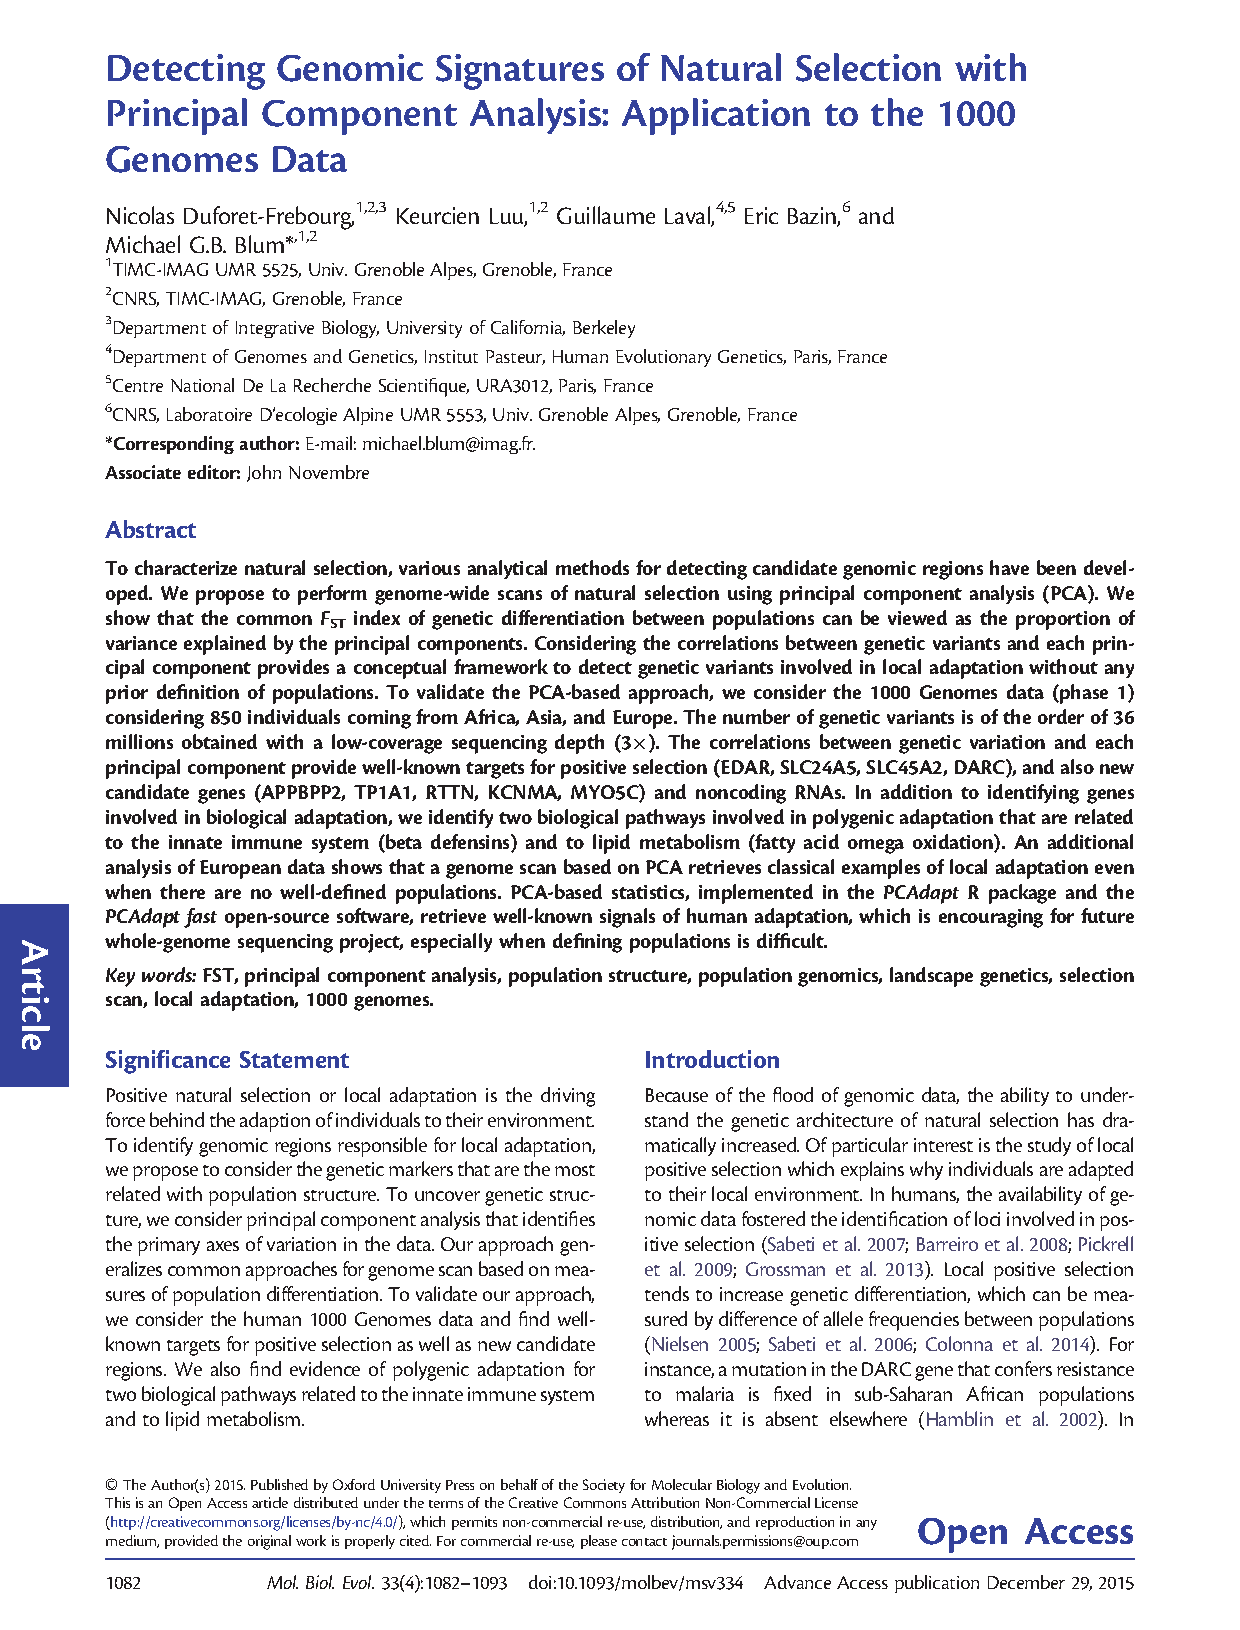
\includepdf[pages=-]{article/msv334.pdf}

\newpage

\section{La distance robuste de
Mahalanobis}\label{la-distance-robuste-de-mahalanobis}

\newpage

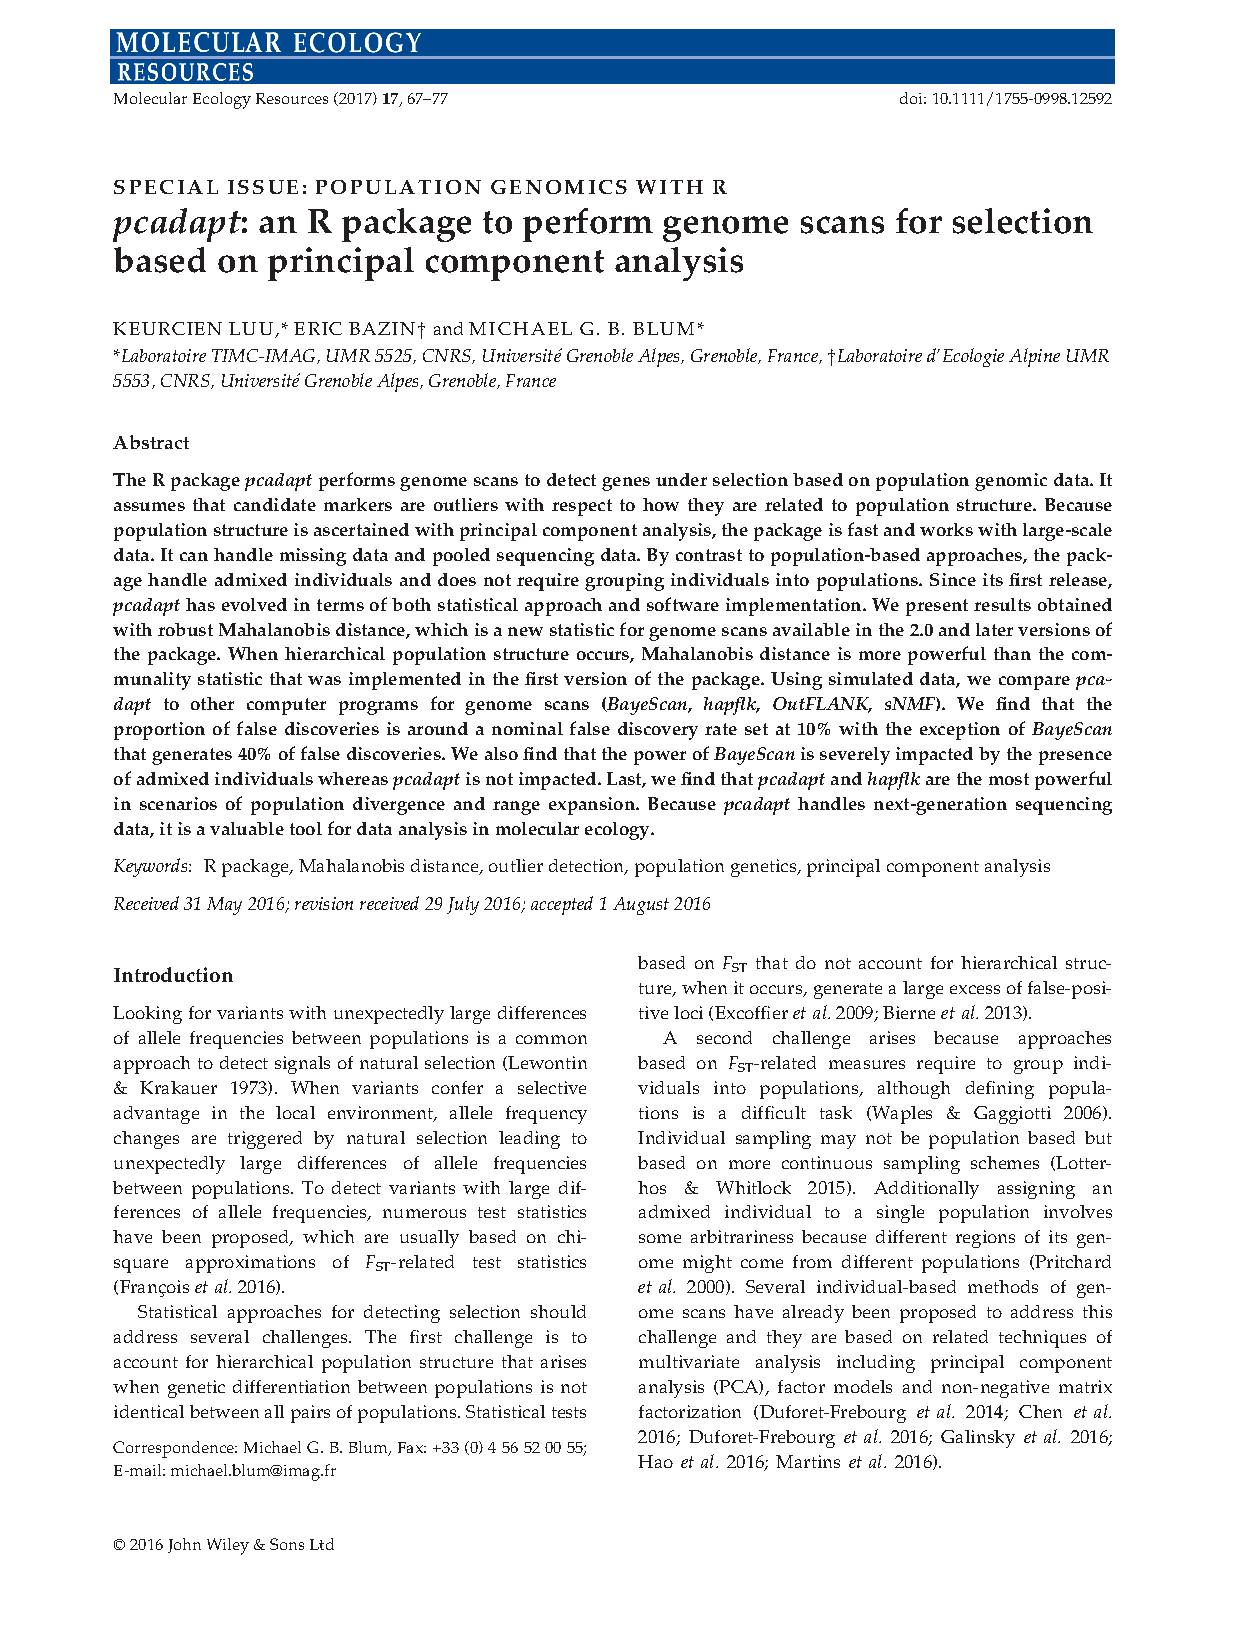
\includepdf[pages=-]{article/Luu_et_al-2017-Molecular_Ecology_Resources.pdf}

\newpage

\chapter{Introgression adaptative}\label{introgression-adaptative}

\section{Qu'est-ce que l'introgression
?}\label{quest-ce-que-lintrogression}

Avant de s'intéresser à la notion d'introgression, intéressons-nous
d'abord à celle d'hybridation. L'hybridation peut être définie comme la
reproduction entre deux individus appartenant à deux espèces ou à deux
populations différentes. Cette définition nous amène à nous poser deux
questions. La première, relative à la notion d'espèce, est souvent
sujette à controverse. La seconde concerne quant à elle la désignation
de populations différentes. Qu'est-ce qui fait que deux groupes
d'individus sont différents ? Harrison suggère en 1990 que deux
individus issus de populations différentes doivent chacun posséder des
traits héritables qui les différencient (Harrison \& others, 1990).

Nous parlons d'introgression lorsqu'un certain nombre de gènes est
transféré d'une population à une autre.

L'étude de régions génomiques présentant des caractéristiques
d'introgression ou de divergence peut se révéler intéressante pour
plusieurs raisons.

\section{Coefficients de métissage globaux et
locaux}\label{coefficients-de-metissage-globaux-et-locaux}

Étant données des populations ancestrales, il est possible d'estimer
pour un individu donné, la proportion de son génôme provenant de chacune
des populations ancestrales. Ces proportions sont connues plus
communément sous le nom de \emph{coefficients de métissage globaux}. De
nombreux logiciels existent pour l'estimation de ces coefficients :
STRUCTURE, ADMIXTURE (Alexander, Novembre, \& Lange, 2009), LEA (Frichot
\& François, 2015), tess3r (Caye, Deist, Martins, Michel, \& François,
2016). En complément à cette information globale, il peut être
intéressant de déterminer sur des portions plus petites du génôme, de la
même manière que dans le cas global, les proportions venant de telle ou
telle population ancestrale pour chacune de ces portions. Nous parlons
dans ce cas de \emph{coefficients de métissage locaux}. Encore une fois,
plusieurs logiciels ont été proposés dans le but d'estimer ces
coefficients : Hapmix (Price et al., 2009), EILA (Yang, Li, Buu, \&
Williams, 2013), LAMP (Thornton \& Bermejo, 2014), loter ou encore RFmix
(Maples, Gravel, Kenny, \& Bustamante, 2013).

\section{Introgression}\label{introgression}

L'introgression peut être détectée de différentes façons. Une première
approche consiste à utiliser les \emph{coefficients de métissage
locaux}. Les méthodes mentionnées plus haut estiment ces coefficients
pour chaque individu, permettant de calculer à partir de ceux-ci des
coefficients de métissage locaux pour chaque population.

\section{Lien entre Analyse en Composantes Principales et métissage
global.}\label{lien-entre-analyse-en-composantes-principales-et-metissage-global.}

L'un des premiers articles à établir un lien entre l'ACP et les
coefficients de métissage global fut sur l'interprétation généalogique
de l'ACP de Gil McVean (McVean, 2009):


\begin{figure}

{\centering 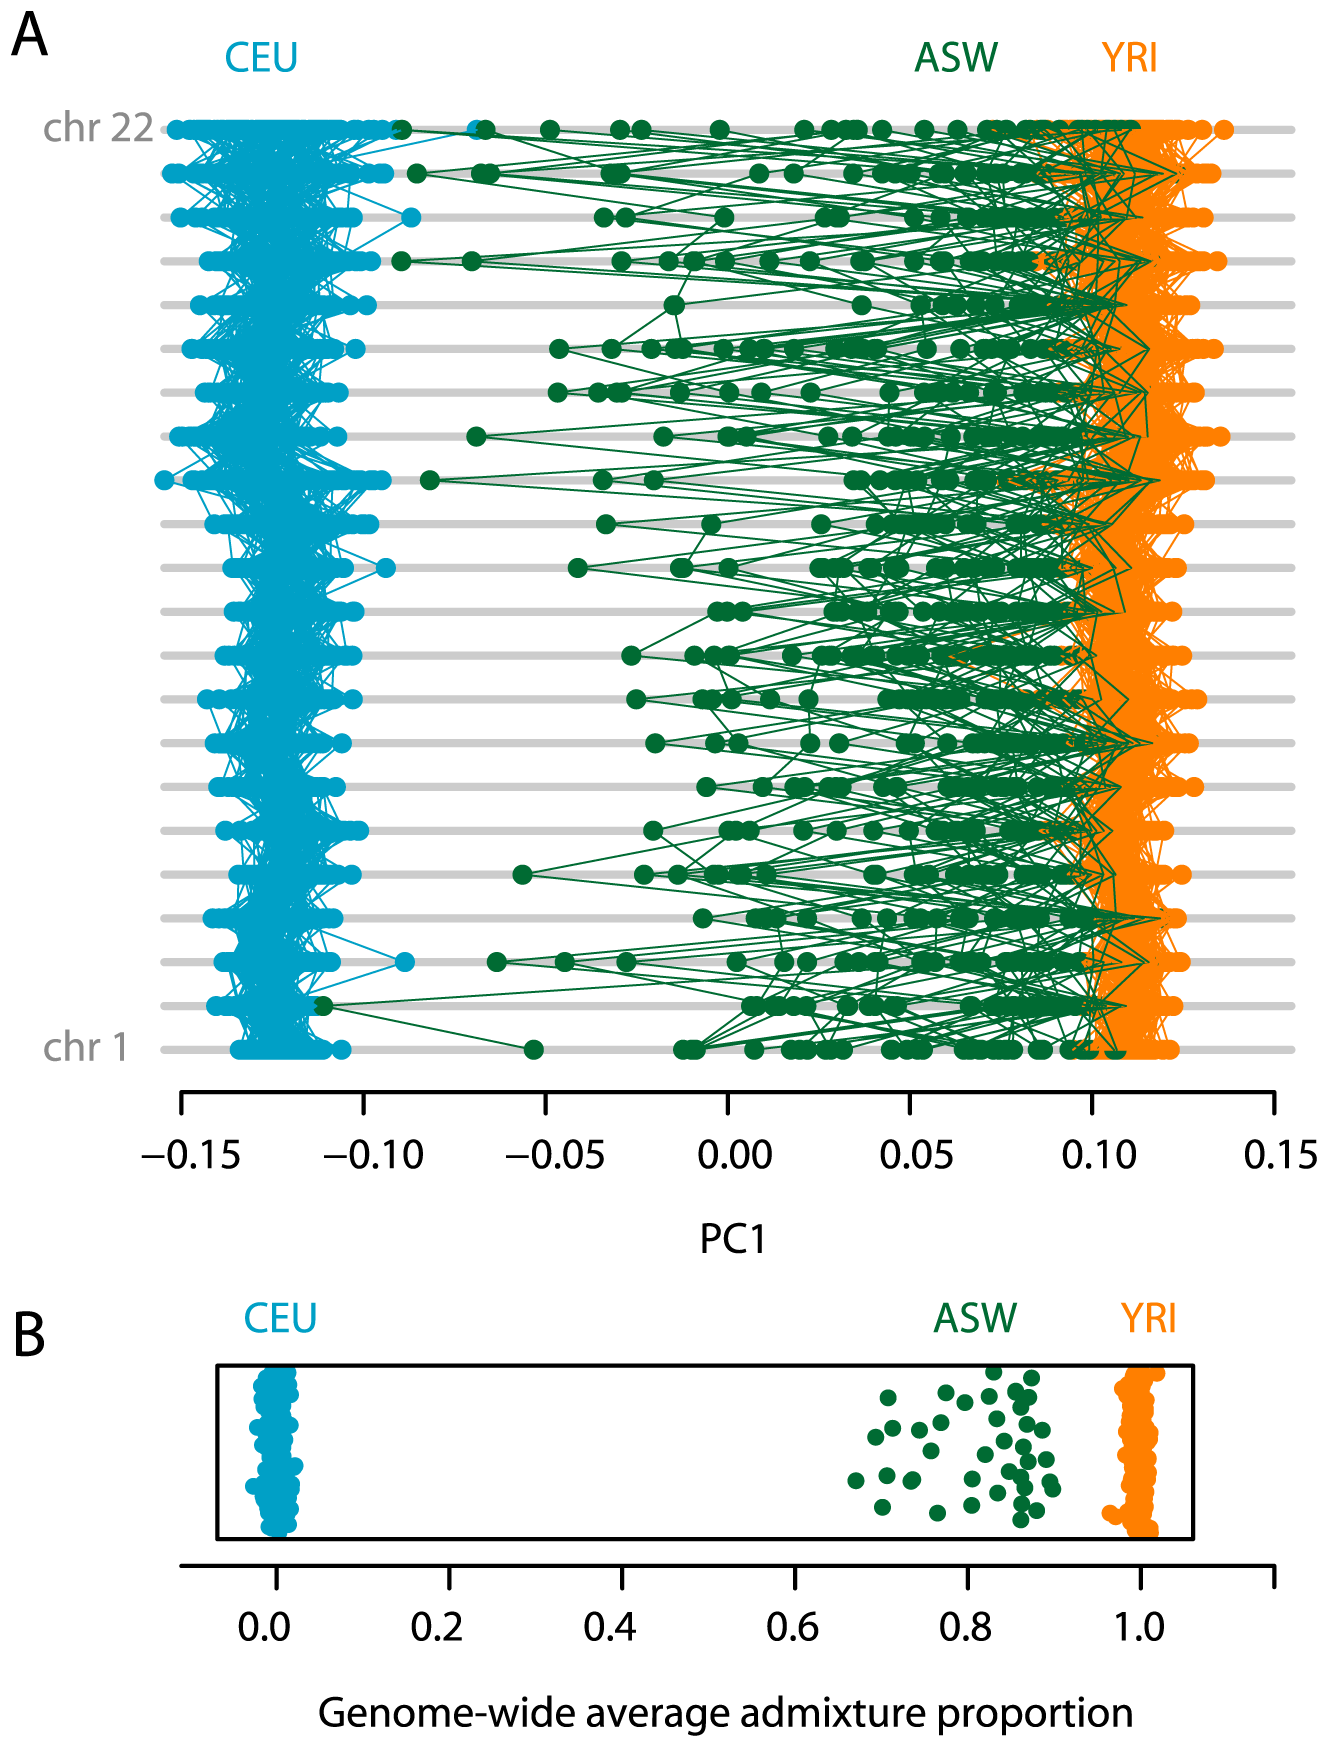
\includegraphics[width=300px]{figure/mcvean} 

}

\caption{Coefficients de métissage et ACP (McVean, 2009).}\label{fig:mcvean}
\end{figure}
Pour chacun des 22 chromosomes,

\section{Analyse en Composantes Principales
locale}\label{analyse-en-composantes-principales-locale}

Notant \(p\) le nombre de marqueurs génétiques, \(i\) un entier compris
entre \(1\) et \(p\), et \(x_i\) la position génétique (en Morgans) ou
la position physique (en paires de bases) du \(i\)-ème marqueur
génétique. Nous définissons pour cet entier \(i\) la fenêtre \(W_i^T\)
de taille \(T\) et centrée en \(i\) :

\[W_i^T = \{ j \in [|1, p|], |x_i - x_j| \leq T/2 \}\]

\section{Sensibilité à l'imputation des données
manquantes}\label{sensibilite-a-limputation-des-donnees-manquantes}

\newpage

\subsection{Méthodes de détection}\label{methodes-de-detection}

\subsubsection{Etat de l'art}\label{etat-de-lart-1}

\paragraph{Scénario à flux de gènes}\label{scenario-a-flux-de-genes}

\subparagraph{La statistique D de
Patterson}\label{la-statistique-d-de-patterson}

La statistique \(D\) de Patterson (Durand, Patterson, Reich, \& Slatkin,
2011) demeure aujourd'hui la méthode la plus utilisée pour détecter la
trace de flux de gènes dans une population. La méthode repose sur
l'observation de motifs portant les noms \emph{ABBA} et \emph{BABA}, en
référence aux différents types de généalogie possible pour un site
nucléotidique.

\[ D = \displaystyle \frac{\sum_i C_{ABBA}(i) - C_{BABA}(i)}{\sum_i C_{ABBA}(i) + C_{BABA}(i)} \]

\subparagraph{RNDmin}\label{rndmin}

{[}Descriptif de RNDmin{]}

Pour comprendre la récente méthode proposée par (Rosenzweig, Pease,
Besansky, \& Hahn, 2016), il est nécessaire de définir un certain nombre
de statistiques dont \(RND_{\text{min}}\) dérive.

~
\begin{itemize}
\tightlist
\item
  \(d_{xy}\) est la distance de Hamming entre la séquence \(X\) de la
  population \(1\) et la séquence \(Y\) de la population \(2\). Ainsi,
  si \(x = (x_i)_{1 \leq i \leq n}\) et \(y = (y_i)_{1 \leq i \leq n}\),
  alors :
\end{itemize}
\[d_{xy} = \text{Card}(\{i \in [|1, n|] \; | \; x_i \neq y_i \})\]

Cette statistique est ainsi définie pour une paire de séquences (\(x\),
\(y\)). Pour quantifier la dissimilarité entre deux ensembles de
séquences, deux approches sont possibles. La première consiste à
calculer la distance moyenne \(d_{XY}\). De par sa définition, cette
distance présente néanmoins le défaut d'être peu sensible aux épisodes
récents d'introgression (Geneva, Muirhead, Kingan, \& Garrigan, 2015).
En effet, les faibles valeurs de \(d_{xy}\) correspondant à des
évènements de divergence récents peuvent voir leur influence diminuée en
cas de présence d'évènements de divergence plus anciens. Pour pallier à
ce problème, considérer la distance minimale entre les deux ensembles de
séquences (Joly, McLenachan, \& Lockhart, 2009) constitue une solution
intéressante.

{[}Expliquer pourquoi on définit \(d_{\text{out}}\) et \(RND\){]}

En définissant \(d_{out} = \frac{1}{2}(d_{XO} + d_{YO})\), il est
possible de définir de la même façon \(RND_{min}\) :

\[RND_{\text{min}} = \frac{d_{\text{min}}}{d_{\text{out}}}\]

Pour récapituler, \(RND_{\text{min}}\) est une statistique robuste aux
variations de taux de mutation et qui reste sensible aux récents
évènements d'introgression. En pratique, l'introduction de
\(d_{\text{out}}\) requiert ainsi la donnée d'une population ancestrale
commune aux deux populations d'intérêt.

\subparagraph{Bdf}\label{bdf}

\paragraph{Analyse Linéaire
Discriminante}\label{analyse-lineaire-discriminante}

\subsubsection{Régression linéaire, régression logistique, forêts
aléatoires et importance des
variables}\label{regression-lineaire-regression-logistique-forets-aleatoires-et-importance-des-variables}

\subsubsection{Régression locale, package mgcv, locfit, Backward
selection
strategy}\label{regression-locale-package-mgcv-locfit-backward-selection-strategy}

\subsubsection{ACP locale et espace de
formes}\label{acp-locale-et-espace-de-formes}

\newpage

\section{Simulations}\label{simulations}

\subsection{Données de peupliers}\label{donnees-de-peupliers}

Le premier jeu de données est issu d'une étude d'introgression
adaptative chez les peupliers d'Amérique du Nord (Suarez-Gonzalez,
2016). La simulation d'haplotypes d'individus admixés est effectuée à
partir des deux populations ancestrales qui y sont présentes. La
première, \emph{Populus Balsamifera}, est une espèce de peupliers qui
peuple le nord du continent nord-américain, d'Est en Ouest, et se trouve
exposée à des conditions climatiques peu clémentes.La seconde,
\emph{Populus Trichocarpa}, est principalement localisée en Californie,
et bénéficie d'un climat continental.

Chacune des simulations est constituée de \(50\) haplotypes de la souche
continentale, de \(50\) haplotyêpes de la souche boréale, ainsi que de
\(50\) haplotypes d'individus hybrides générés à partir des haplotypes
ancestraux. Ces haplotypes ancestraux ont été estimés à l'aide du
logiciel Beagle. A partir des positions en paires de base, une carte de
recombinaison génétique est générée en utilisant le taux de
recombinaison moyen chez le peuplier. Le taux de recombinaison, noté
\(\tau_r\), correspond au nombre moyen de paires de bases à parcourir
pour qu'ait lieu un épisode de recombinaison génétique, \emph{i.e.},
notant \(L\) la longueur du chromosome en Morgans (\(M\)), et \(N_{bp}\)
le nombre de paires de bases le constituant, le taux de recombinaison
génétique pour ce chromosome est donné par la relation:

\[\tau_r = \frac{L}{N_{bp}}\]

Dans ce scénario, les simulations ont été produites en utilisant un taux
de recombinaison génétique moyen \(\tau_r\) de \(0.05\) centiMorgans par
million de paire de bases, correspondant à la valeur utilisée par les
auteurs de l'étude avec le logiciel RASPberry
(\textit{Recombination via Ancestry Switch Probability}). A partir de la
donnée de la position physique en paires de bases ainsi que du taux de
recombinaison moyen, nous générons une carte de recombinaison génétique
adaptée à nos simulations.

\subsection{Génération aléatoire d'individus
hybrides}\label{generation-aleatoire-dindividus-hybrides}

Pour simuler un individu métissé, il est d'abord nécessaire de simuler
l'emplacement des évènements de recombinaison. Pour ce faire, nous
utilisons le modèle décrit dans (Price et al., 2009), en parcourant

\newpage

\subsection{Simulations à partir de ms et
Seq-Gen}\label{simulations-a-partir-de-ms-et-seq-gen}

Dans le scénario d'introgression via flux de gènes, nous nous inspirons
des modèles de simulation décrits dans (Martin \& Jiggins, 2015). Ces
modèles sont largement repris dans la littérature pour l'évaluation de
statistiques telles que \(RND_{min}\) (Rosenzweig et al., 2016) et
\(Bd_f\) (Pfeifer \& Kapan, 2017). Chaque simulation est constituée de
100 individus. Un individu est généré en concaténant un certain nombre
de séquences de nucléotides, d'une longueur fixée à 5000 paires de bases
par séquence. Chacune de ces séquences est elle-même simulée suivant un
modèle neutre ou alternatif. Le modèle neutre décrit un scénario
démographique classique de populations divergentes. Le modèle alternatif
décrit quant à lui un scénario légèrement différent, et servira à
caractériser les séquences \emph{introgressées}. Les lignes de commande
\emph{ms} permettant de générer les séquences de nucléotides pour le
modèle neutre ainsi que pour le modèle alternatif sont données
ci-dessous :

~
\begin{itemize}
\tightlist
\item
  Modèle neutre :
\end{itemize}
\begin{verbatim}
./ms 200 1 -I 4 50 50 50 50 -ej 1 2 1 -ej 2 3 1 -ej 3 4 1 
-r 50 5000 -T 
\end{verbatim}
\begin{figure}

{\centering 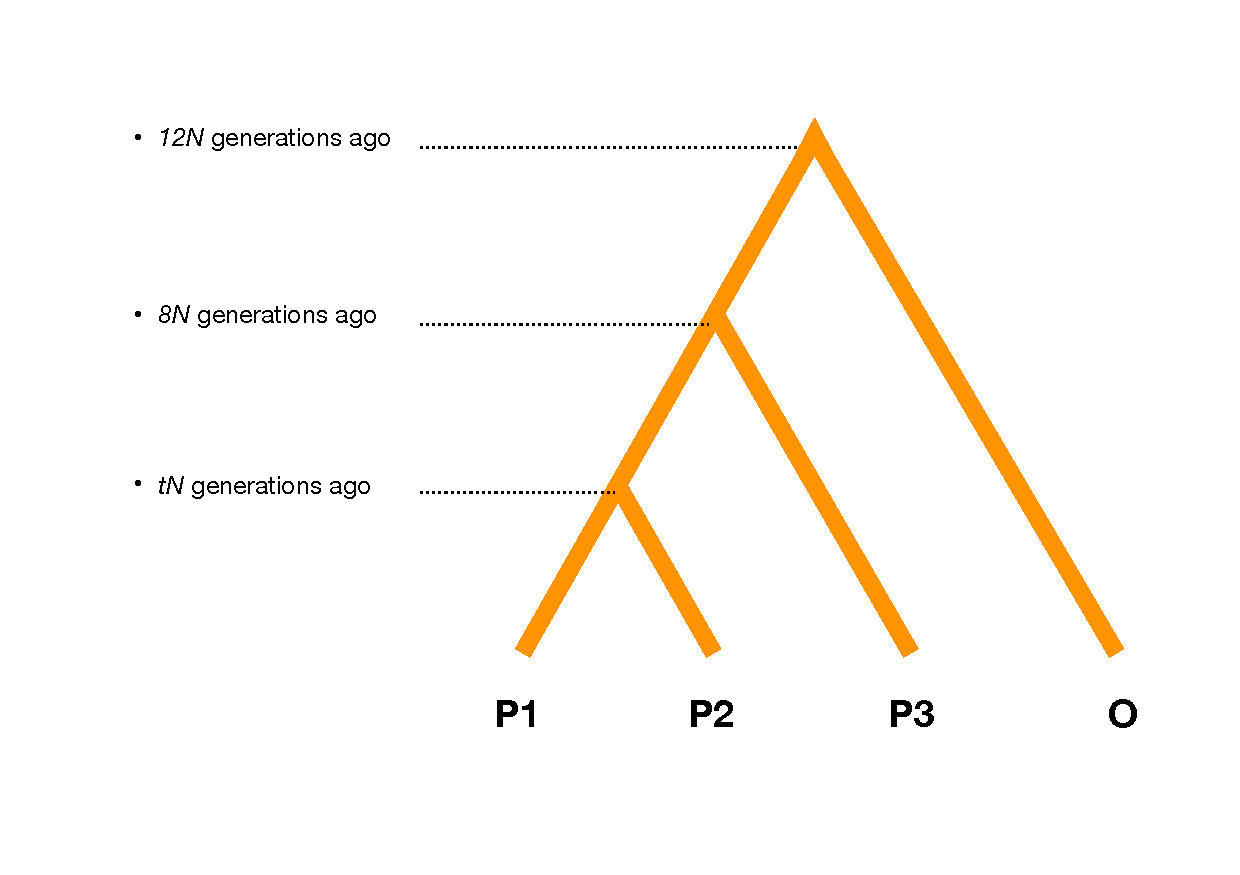
\includegraphics[scale=0.5]{figure/background} 

}

\caption{Modèle neutre. $12N$ genérations auparavant, premier épisode de divergence donnant naissance à P1 et à O. $8N$ générations auparavant, deuxième épisode de divergence voyant l'apparition de P3. $4N$ générations auparavant, dernier épisode de divergence et apparition de P2.}\label{fig:background}
\end{figure}
~
\begin{itemize}
\tightlist
\item
  Modèle alternatif :
\end{itemize}
\begin{verbatim}
./ms 200 1 -I 4 50 50 50 50 -ej 1 2 1 -ej 2 3 1 -ej 3 4 1 
-es 0.1 2 0.8 -ej 0.1 5 3 -r 50 5000 -T
\end{verbatim}
\begin{figure}

{\centering 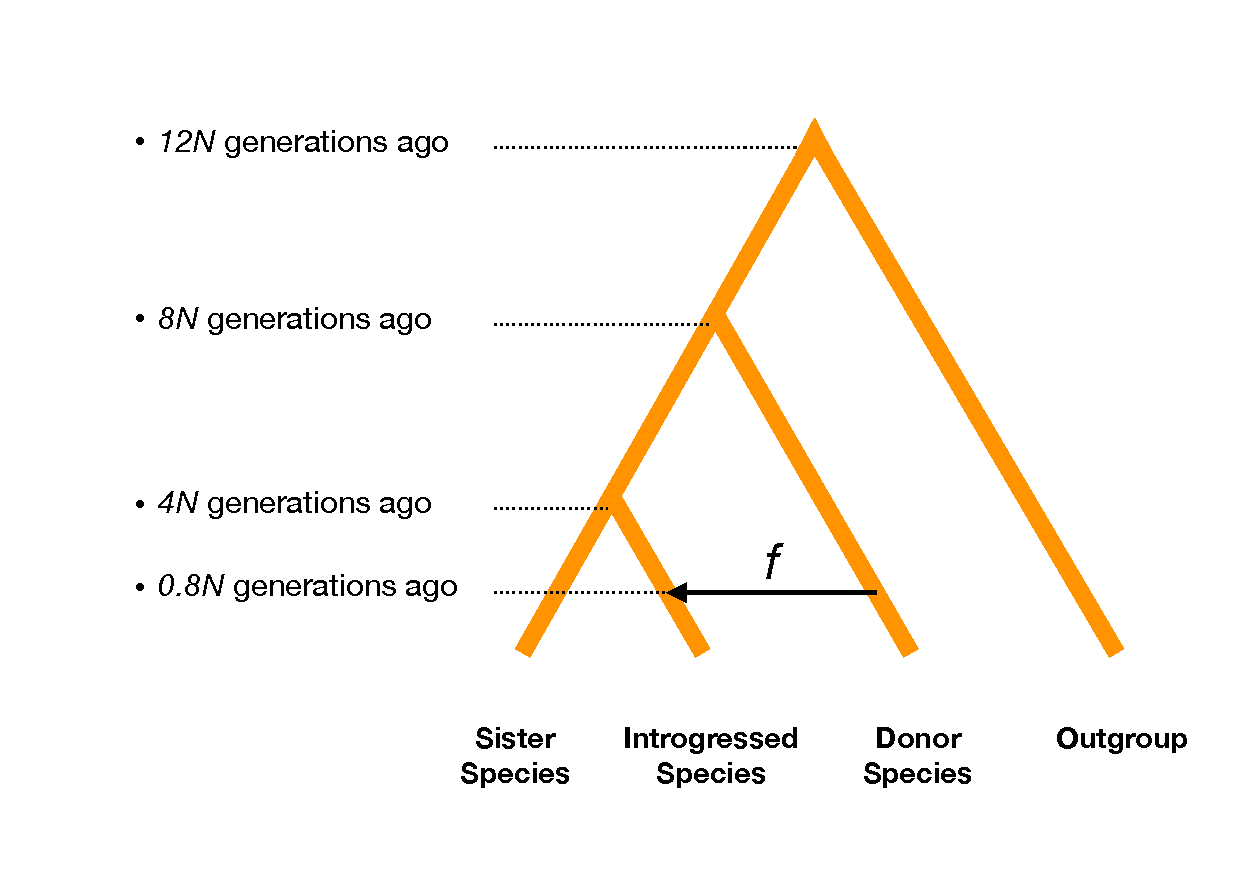
\includegraphics[scale=0.5]{figure/alternate} 

}

\caption{Modèle alternatif. $12N$ genérations auparavant, premier épisode de divergence donnant naissance à P1 et à O. $8N$ générations auparavant, deuxième épisode de divergence voyant l'apparition de P3. $4N$ générations auparavant, dernier épisode de divergence et apparition de P2. $t$ unités de temps auparavant, épisode de flux de gènes de P3 vers la population P2.}\label{fig:alternate}
\end{figure}
La variable \(f\) présente en figure \ref{fig:alternate} représente le
taux d'introgression, elle quantifie la proportion d'haplotypes présents
dans la population P2 et qui proviennent de la population P3. Ainsi, une
valeur de \(f\) égale à \(1\) reviendrait à simuler un épisode de
divergence de la population P3, duquel découlerait la naissance de la
population P2. La valeur de \(f\) utilisée ci-dessus est \(0.2\),
signifiant que 20\% des haplotypes présents dans la population 2 sont
issus de la population P3.

\subsection{Résultats de la comparaison des
logiciels}\label{resultats-de-la-comparaison-des-logiciels}

\paragraph{Scénario de métissage}\label{scenario-de-metissage}

Nous comparons ici notre méthode au logiciel RFMix destiné à la
détermination de coefficients de métissage local.
\begin{figure}

{\centering 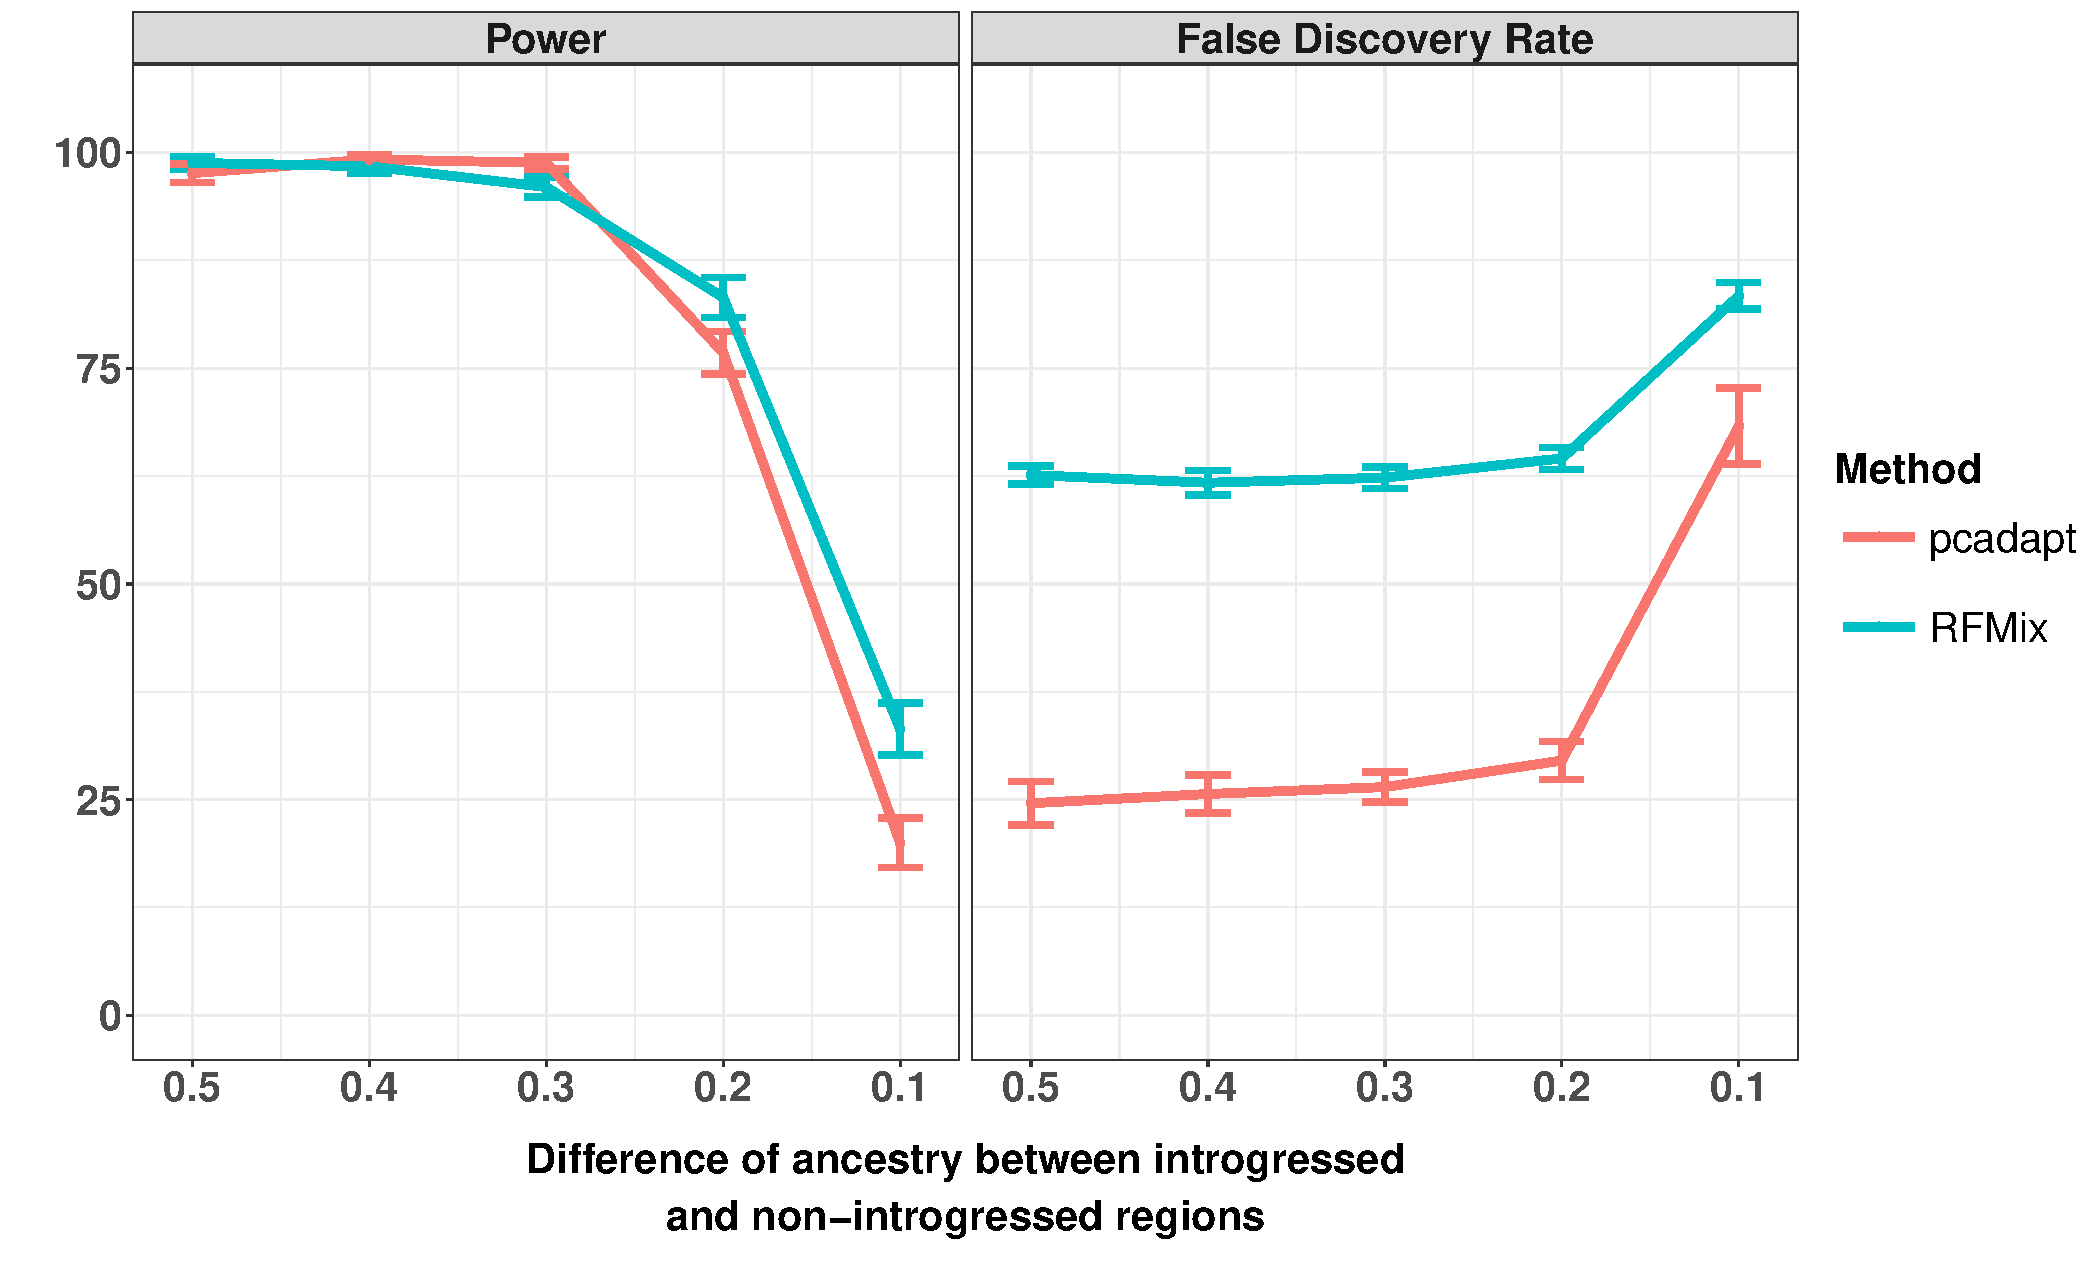
\includegraphics[width=500px]{figure/facet_admixture_setting_10_gen} 

}

\caption{10 generations}\label{fig:ras10g}
\end{figure}
\begin{figure}

{\centering 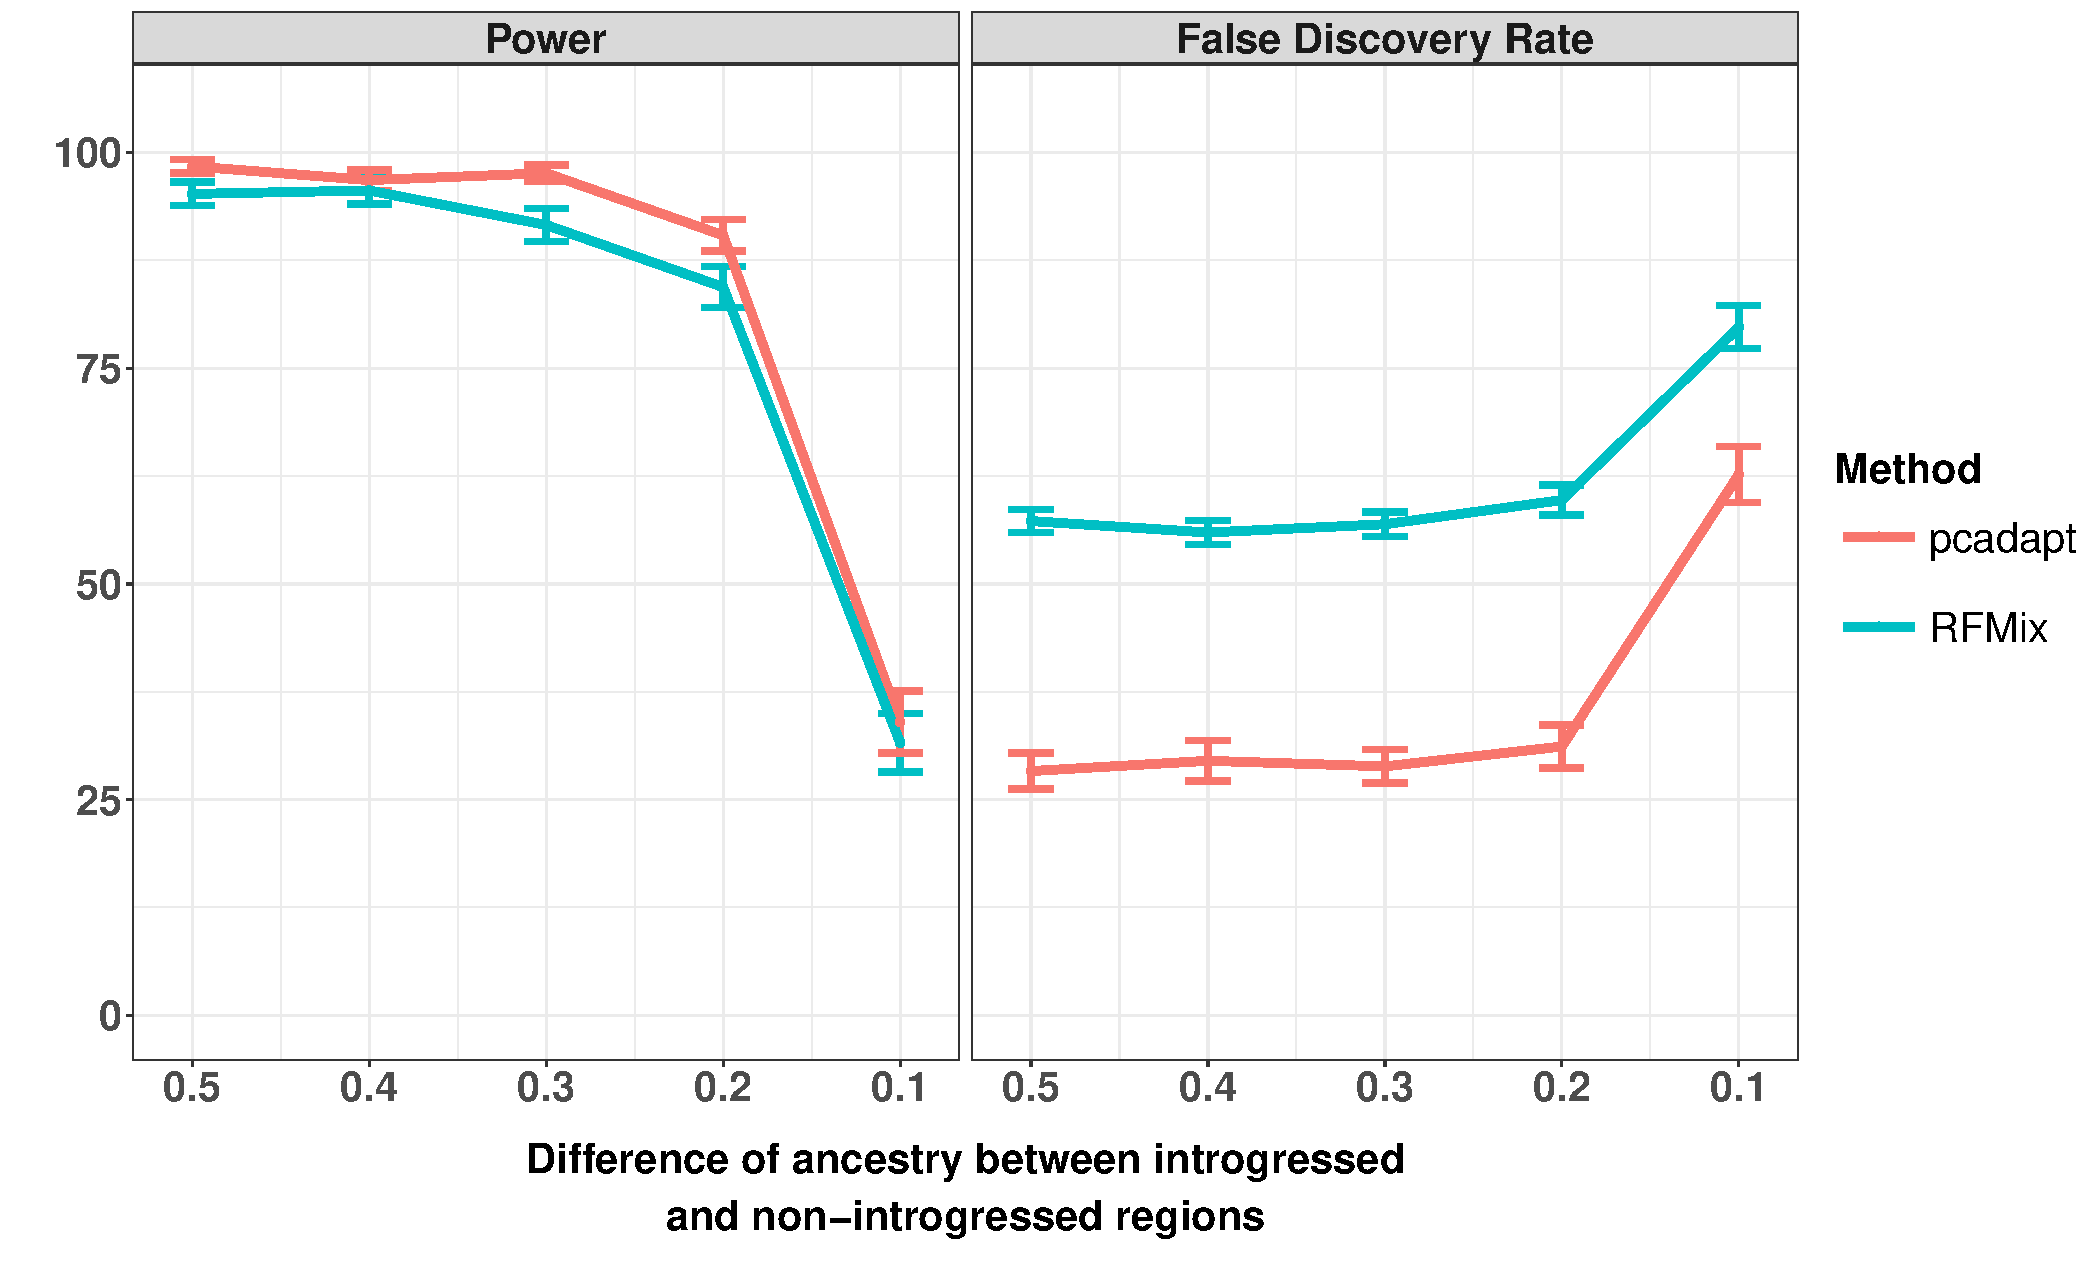
\includegraphics[width=500px]{figure/facet_admixture_setting_100_gen} 

}

\caption{100 generations}\label{fig:ras100g}
\end{figure}
\begin{figure}

{\centering 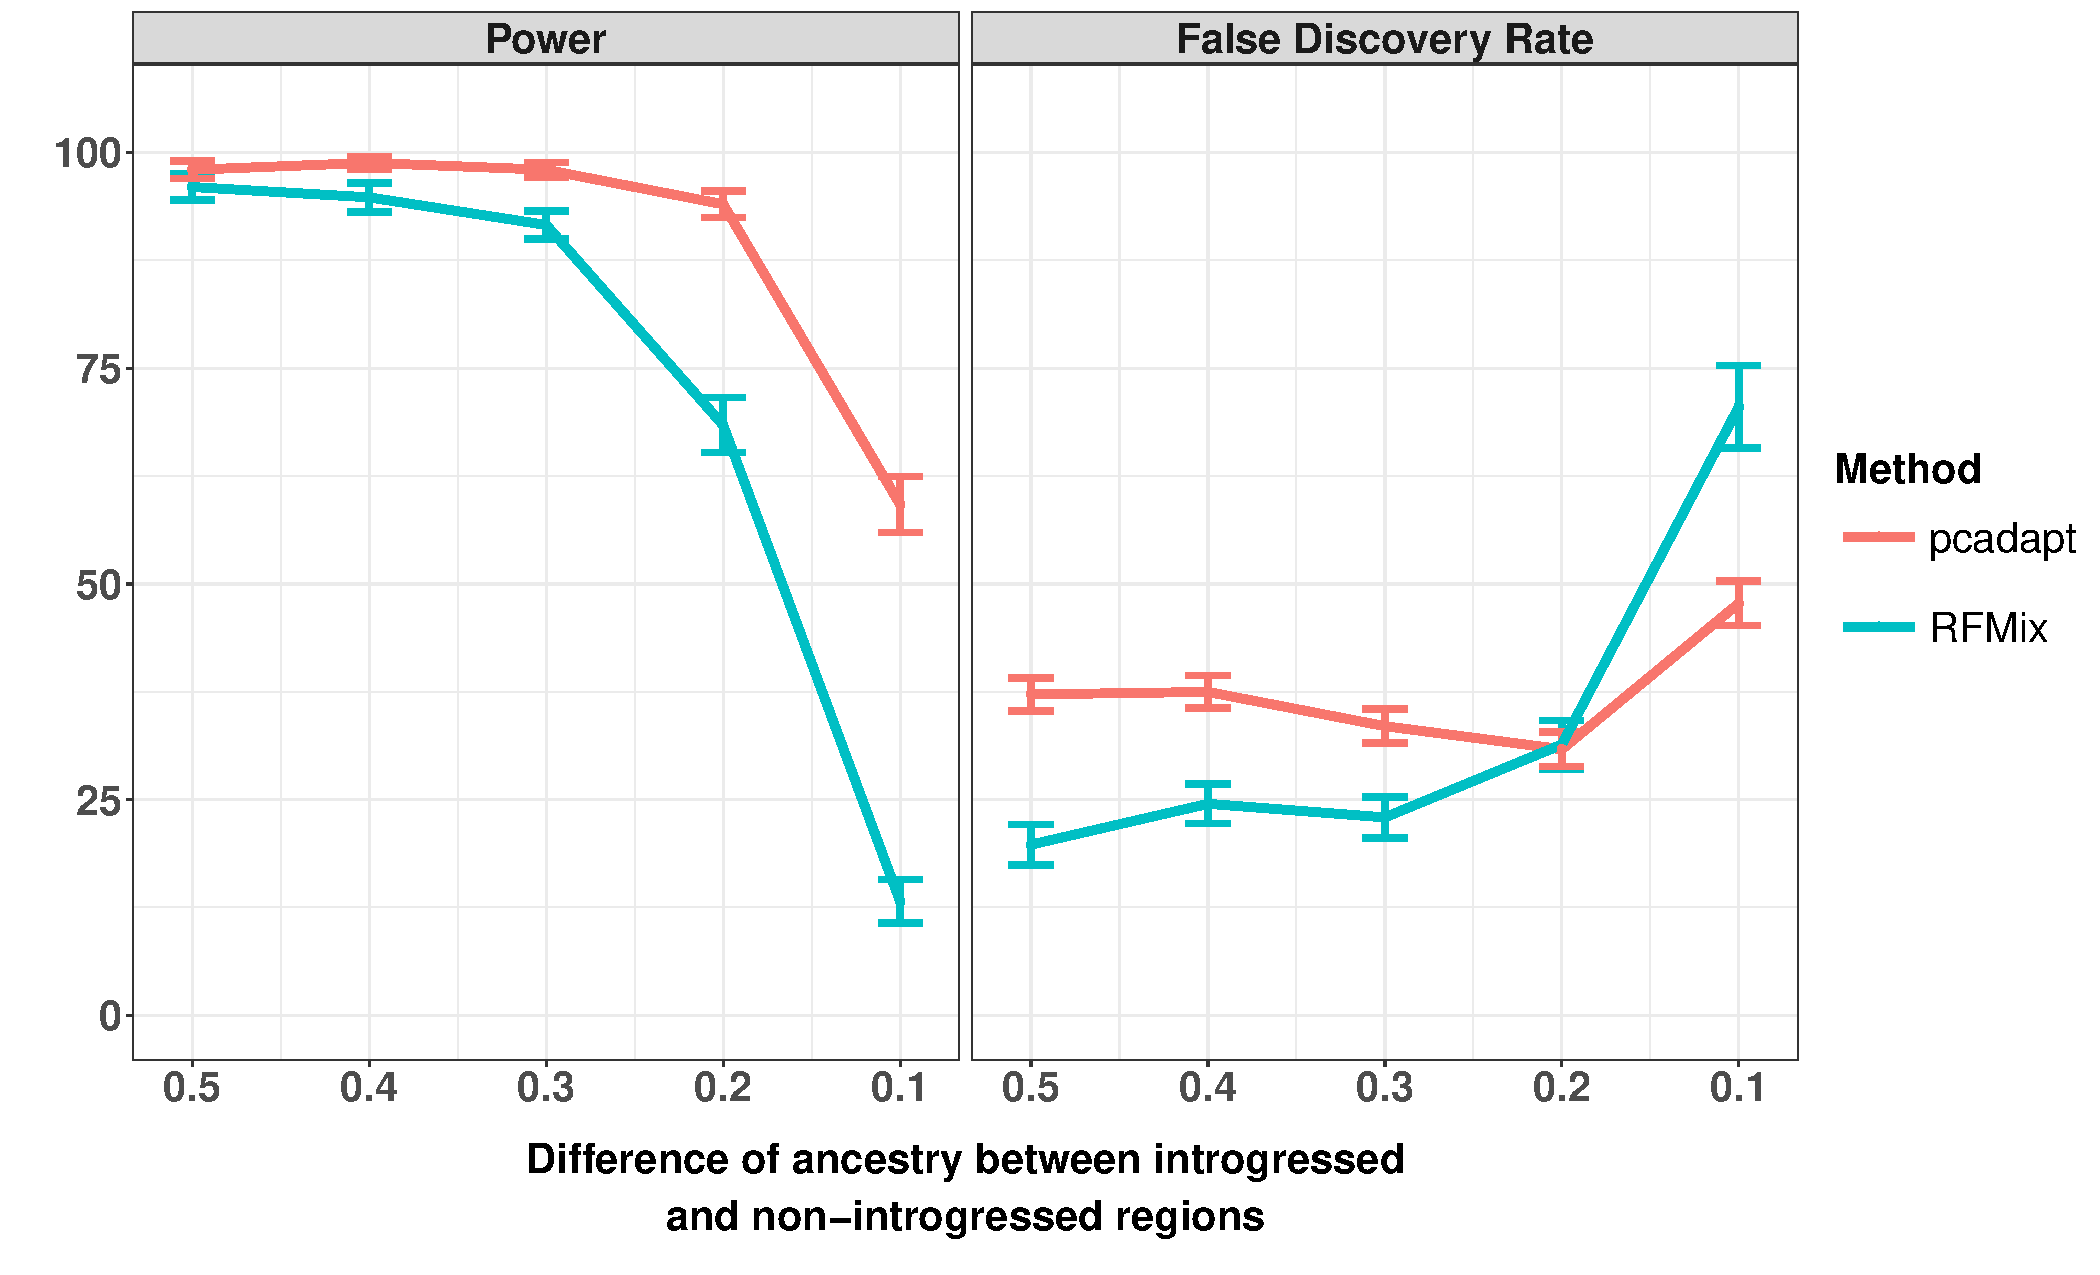
\includegraphics[width=500px]{figure/facet_admixture_setting_1000_gen} 

}

\caption{1000 generations}\label{fig:ras1000g}
\end{figure}
\paragraph{Scénario à flux de gènes}\label{scenario-a-flux-de-genes-1}

Dans ce paragraphe, nous comparons notre statistique de test à un
ensemble de statistiques implémentées dans le package R \emph{PopGenome}
: la statistique \(D\) de Patterson, RNDmin (Rosenzweig et al., 2016) et
BDF (Pfeifer \& Kapan, 2017).

\chapter{Aspect computationnel}\label{aspect-computationnel}

Dans cette partie, nous nous intéresserons brièvement à l'aspect
computationnel des méthodes qui ont été présentées dans les chapitres
précédents. Le développement d'outils logiciels destinés à l'exploration
de données génétiques volumineuses requiert qu'une attention toute
particulière soit portée à l'utilisation des ressources de calcul.

Blockwise computation of covariance matrix Random SVD Storage in binary
format Memory-mapping

Pairwise-Cor (Dray \& Josse, 2015)

\chapter*{Conclusion}\label{conclusion}
\addcontentsline{toc}{chapter}{Conclusion}

If we don't want Conclusion to have a chapter number next to it, we can
add the \texttt{\{-\}} attribute.

\textbf{More info}

And here's some other random info: the first paragraph after a chapter
title or section head \emph{shouldn't be} indented, because indents are
to tell the reader that you're starting a new paragraph. Since that's
obvious after a chapter or section title, proper typesetting doesn't add
an indent there.

\appendix

\chapter{The First Appendix}\label{the-first-appendix}

This first appendix includes all of the R chunks of code that were
hidden throughout the document (using the \texttt{include\ =\ FALSE}
chunk tag) to help with readibility and/or setup.

\textbf{In the main Rmd file}
\begin{Shaded}
\begin{Highlighting}[]
\NormalTok{if(!}\KeywordTok{require}\NormalTok{(devtools)) \{}
  \KeywordTok{install.packages}\NormalTok{(}\StringTok{"devtools"}\NormalTok{, }\DataTypeTok{repos =} \StringTok{"http://cran.rstudio.com"}\NormalTok{)}
\NormalTok{\}}

\NormalTok{if(!}\KeywordTok{require}\NormalTok{(dplyr)) \{}
  \KeywordTok{install.packages}\NormalTok{(}\StringTok{"dplyr"}\NormalTok{, }\DataTypeTok{repos =} \StringTok{"http://cran.rstudio.com"}\NormalTok{)}
\NormalTok{\}}

\NormalTok{if(!}\KeywordTok{require}\NormalTok{(ggplot2)) \{}
  \KeywordTok{install.packages}\NormalTok{(}\StringTok{"ggplot2"}\NormalTok{, }\DataTypeTok{repos =} \StringTok{"http://cran.rstudio.com"}\NormalTok{)}
\NormalTok{\}}

\NormalTok{if(!}\KeywordTok{require}\NormalTok{(bookdown)) \{}
  \KeywordTok{install.packages}\NormalTok{(}\StringTok{"bookdown"}\NormalTok{, }\DataTypeTok{repos =} \StringTok{"http://cran.rstudio.com"}\NormalTok{)}
\NormalTok{\}}

\NormalTok{if(!}\KeywordTok{require}\NormalTok{(thesisdown)) \{}
  \NormalTok{devtools::}\KeywordTok{install_github}\NormalTok{(}\StringTok{"ismayc/thesisdown"}\NormalTok{)}
\NormalTok{\}}

\NormalTok{if(!}\KeywordTok{require}\NormalTok{(data.table)) \{}
  \KeywordTok{install.packages}\NormalTok{(}\StringTok{"data.table"}\NormalTok{, }\DataTypeTok{repos =} \StringTok{"http://cran.rstudio.com"}\NormalTok{)}
\NormalTok{\}}

\NormalTok{if(!}\KeywordTok{require}\NormalTok{(pcadapt)) \{}
  \NormalTok{devtools::}\KeywordTok{install_github}\NormalTok{(}\StringTok{"bcm-uga/pcadapt"}\NormalTok{)}
\NormalTok{\}}

\NormalTok{if(!}\KeywordTok{require}\NormalTok{(simulate)) \{}
  \NormalTok{devtools::}\KeywordTok{install_github}\NormalTok{(}\StringTok{"keurcien/simulate"}\NormalTok{)}
\NormalTok{\}}

\NormalTok{if(!}\KeywordTok{require}\NormalTok{(kableExtra))\{}
  \KeywordTok{install.packages}\NormalTok{(}\StringTok{"kableExtra"}\NormalTok{)}
\NormalTok{\}}

\NormalTok{if(!}\KeywordTok{require}\NormalTok{(maps))\{}
  \KeywordTok{install.packages}\NormalTok{(}\StringTok{"maps"}\NormalTok{)}
\NormalTok{\}}

\NormalTok{knitr::opts_chunk$}\KeywordTok{set}\NormalTok{(}\DataTypeTok{echo =} \OtherTok{FALSE}\NormalTok{,}
                      \DataTypeTok{fig.align =} \StringTok{'center'}\NormalTok{,}
                      \DataTypeTok{fig.width =} \DecValTok{6}\NormalTok{,}
                      \DataTypeTok{results =} \StringTok{'hide'}\NormalTok{)}

\CommentTok{# knitr::opts_chunk$set(cache = TRUE)}

\CommentTok{# The palette with black:}
\NormalTok{cbbPalette <-}\StringTok{ }\KeywordTok{c}\NormalTok{(}\StringTok{"#000000"}\NormalTok{, }
                \StringTok{"#E69F00"}\NormalTok{, }
                \StringTok{"#56B4E9"}\NormalTok{, }
                \StringTok{"#009E73"}\NormalTok{, }
                \StringTok{"#F0E442"}\NormalTok{, }
                \StringTok{"#0072B2"}\NormalTok{, }
                \StringTok{"#D55E00"}\NormalTok{, }
                \StringTok{"#CC79A7"}\NormalTok{)}
\end{Highlighting}
\end{Shaded}
\chapter{The Second Appendix, for
Fun}\label{the-second-appendix-for-fun}

\backmatter

\chapter*{Bibliographie}\label{bibliographie}
\addcontentsline{toc}{chapter}{Bibliographie}

\noindent

\setlength{\parindent}{-0.20in} \setlength{\leftskip}{0.20in}
\setlength{\parskip}{8pt}

\hypertarget{refs}{}
\hypertarget{ref-alexander2009fast}{}
Alexander, D. H., Novembre, J., \& Lange, K. (2009). Fast model-based
estimation of ancestry in unrelated individuals. \emph{Genome Research},
\emph{19}(9), 1655--1664.

\hypertarget{ref-bateson1913mendel}{}
Bateson, W., \& Mendel, G. (1913). \emph{Mendel's principles of
heredity}. University press.

\hypertarget{ref-beaumont2004identifying}{}
Beaumont, M. A., \& Balding, D. J. (2004). Identifying adaptive genetic
divergence among populations from genome scans. \emph{Molecular
Ecology}, \emph{13}(4), 969--980.

\hypertarget{ref-bonhomme2010detecting}{}
Bonhomme, M., Chevalet, C., Servin, B., Boitard, S., Abdallah, J.,
Blott, S., \& SanCristobal, M. (2010). Detecting selection in population
trees: The lewontin and krakauer test extended. \emph{Genetics},
\emph{186}(1), 241--262.

\hypertarget{ref-bromham2003modern}{}
Bromham, L., \& Penny, D. (2003). The modern molecular clock.
\emph{Nature Reviews. Genetics}, \emph{4}(3), 216.

\hypertarget{ref-cavalli1994francesco}{}
Cavalli-Sforza, L. (1994). Francesco. qui sommes-nous? Une histoire de
diversité humaine. \emph{Trans. Brun, Françoise. Flammarion Ed. Paris:
Centre National Des Lettres}.

\hypertarget{ref-caye2016tess3}{}
Caye, K., Deist, T. M., Martins, H., Michel, O., \& François, O. (2016).
TESS3: Fast inference of spatial population structure and genome scans
for selection. \emph{Molecular Ecology Resources}, \emph{16}(2),
540--548.

\hypertarget{ref-charlesworth2009darwin}{}
Charlesworth, B., \& Charlesworth, D. (2009). Darwin and genetics.
\emph{Genetics}, \emph{183}(3), 757--766.

\hypertarget{ref-darwin1980origine}{}
Darwin, C. (1980). L'Origine des espèces, trad. \emph{Edmond Barbier
(1876), Paris, Maspero}.

\hypertarget{ref-dray2015principal}{}
Dray, S., \& Josse, J. (2015). Principal component analysis with missing
values: A comparative survey of methods. \emph{Plant Ecology},
\emph{216}(5), 657--667.

\hypertarget{ref-durand2011testing}{}
Durand, E. Y., Patterson, N., Reich, D., \& Slatkin, M. (2011). Testing
for ancient admixture between closely related populations.
\emph{Molecular Biology and Evolution}, \emph{28}(8), 2239--2252.

\hypertarget{ref-frichot2015lea}{}
Frichot, E., \& François, O. (2015). LEA: An r package for landscape and
ecological association studies. \emph{Methods in Ecology and Evolution},
\emph{6}(8), 925--929.

\hypertarget{ref-gayon1992darwin}{}
Gayon, J. (1992). Darwin et l'après-darwin: Une histoire de l'hypothèse
de sélection dans la théorie de l'évolution. Kimé.

\hypertarget{ref-geneva2015new}{}
Geneva, A. J., Muirhead, C. A., Kingan, S. B., \& Garrigan, D. (2015). A
new method to scan genomes for introgression in a secondary contact
model. \emph{PloS One}, \emph{10}(4), e0118621.

\hypertarget{ref-gillespie2010population}{}
Gillespie, J. H. (2010). \emph{Population genetics: A concise guide}.
JHU Press.

\hypertarget{ref-giraud2014introduction}{}
Giraud, C. (2014). \emph{Introduction to high-dimensional statistics}
(Vol. 138). CRC Press.

\hypertarget{ref-gogol2012overview}{}
Gogol-Döring, A., \& Chen, W. (2012). An overview of the analysis of
next generation sequencing data. \emph{Next Generation Microarray
Bioinformatics: Methods and Protocols}, 249--257.

\hypertarget{ref-harrison1990hybrid}{}
Harrison, R. G., \& others. (1990). Hybrid zones: Windows on
evolutionary process. \emph{Oxford Surveys in Evolutionary Biology},
\emph{7}, 69--128.

\hypertarget{ref-jeong2014adaptations}{}
Jeong, C., \& Di Rienzo, A. (2014). Adaptations to local environments in
modern human populations. \emph{Current Opinion in Genetics \&
Development}, \emph{29}, 1--8.

\hypertarget{ref-joly2009statistical}{}
Joly, S., McLenachan, P. A., \& Lockhart, P. J. (2009). A statistical
approach for distinguishing hybridization and incomplete lineage
sorting. \emph{The American Naturalist}, \emph{174}(2), E54--E70.

\hypertarget{ref-kimura1983neutral}{}
Kimura, M. (1983). \emph{The neutral theory of molecular evolution}.
Cambridge University Press.

\hypertarget{ref-lewontin1973distribution}{}
Lewontin, R., \& Krakauer, J. (1973). Distribution of gene frequency as
a test of the theory of the selective neutrality of polymorphisms.
\emph{Genetics}, \emph{74}(1), 175--195.

\hypertarget{ref-maples2013rfmix}{}
Maples, B. K., Gravel, S., Kenny, E. E., \& Bustamante, C. D. (2013).
RFMix: A discriminative modeling approach for rapid and robust
local-ancestry inference. \emph{The American Journal of Human Genetics},
\emph{93}(2), 278--288.

\hypertarget{ref-martin2000}{}
Martin, J. W. D., Simon H., \& Jiggins, C. D. (2015). Evaluating the use
of abba--BABA statistics to locate introgressed loci. \emph{Molecular
Biology and Evolution}, 244--257.

\hypertarget{ref-mcvean2009genealogical}{}
McVean, G. (2009). A genealogical interpretation of principal components
analysis. \emph{PLoS Genetics}, \emph{5}(10), e1000686.

\hypertarget{ref-menozzi1978synthetic}{}
Menozzi, P., Piazza, A., \& Cavalli-Sforza, L. (1978). Synthetic maps of
human gene frequencies in europeans. \emph{Science}, \emph{201}(4358),
786--792.

\hypertarget{ref-muir2016real}{}
Muir, P., Li, S., Lou, S., Wang, D., Spakowicz, D. J., Salichos, L.,
\ldots{} others. (2016). The real cost of sequencing: Scaling
computation to keep pace with data generation. \emph{Genome Biology},
\emph{17}(1), 53.

\hypertarget{ref-nicholson2002assessing}{}
Nicholson, G., Smith, A. V., Jónsson, F., Gústafsson, Ó., Stefánsson,
K., \& Donnelly, P. (2002). Assessing population differentiation and
isolation from single-nucleotide polymorphism data. \emph{Journal of the
Royal Statistical Society: Series B (Statistical Methodology)},
\emph{64}(4), 695--715.

\hypertarget{ref-novembre2008genes}{}
Novembre, J., Johnson, T., Bryc, K., Kutalik, Z., Boyko, A. R., Auton,
A., \ldots{} others. (2008). Genes mirror geography within europe.
\emph{Nature}, \emph{456}(7218), 98.

\hypertarget{ref-peng2005simupop}{}
Peng, B., \& Kimmel, M. (2005). SimuPOP: A forward-time population
genetics simulation environment. \emph{Bioinformatics}, \emph{21}(18),
3686--3687.

\hypertarget{ref-pfeifer2017estimates}{}
Pfeifer, B., \& Kapan, D. D. (2017). Estimates of introgression as a
function of pairwise distances. \emph{BioRxiv}, 154377.

\hypertarget{ref-price2009sensitive}{}
Price, A. L., Tandon, A., Patterson, N., Barnes, K. C., Rafaels, N.,
Ruczinski, I., \ldots{} Myers, S. (2009). Sensitive detection of
chromosomal segments of distinct ancestry in admixed populations.
\emph{PLoS Genetics}, \emph{5}(6), e1000519.

\hypertarget{ref-roll2014holist}{}
Roll-Hansen, N. (2014). The holist tradition in twentieth century
genetics. wilhelm johannsen's genotype concept. \emph{The Journal of
Physiology}, \emph{592}(11), 2431--2438.

\hypertarget{ref-rosenzweig2016powerful}{}
Rosenzweig, B. K., Pease, J. B., Besansky, N. J., \& Hahn, M. W. (2016).
Powerful methods for detecting introgressed regions from population
genomic data. \emph{Molecular Ecology}, \emph{25}(11), 2387--2397.

\hypertarget{ref-roux2012recent}{}
Roux, C., Pauwels, M., Ruggiero, M.-V., Charlesworth, D., Castric, V.,
\& Vekemans, X. (2012). Recent and ancient signature of balancing
selection around the s-locus in arabidopsis halleri and a. lyrata.
\emph{Molecular Biology and Evolution}, \emph{30}(2), 435--447.

\hypertarget{ref-suarez2016}{}
Suarez-Gonzalez, et a., Adriana. (2016). Genomic and functional
approaches reveal a case of adaptive introgression from populus
balsamifera (balsam poplar) in p. trichocarpa (black cottonwood).
\emph{Molecular Ecology}, 2427--2442.

\hypertarget{ref-thornton2014local}{}
Thornton, T. A., \& Bermejo, J. L. (2014). Local and global ancestry
inference and applications to genetic association analysis for admixed
populations. \emph{Genetic Epidemiology}, \emph{38}(S1).

\hypertarget{ref-wetterstrand2013dna}{}
Wetterstrand, K. A. (2013). DNA sequencing costs: Data from the nhgri
genome sequencing program (gsp).

\hypertarget{ref-whitlock2015reliable}{}
Whitlock, M. C., \& Lotterhos, K. E. (2015). Reliable detection of loci
responsible for local adaptation: Inference of a null model through
trimming the distribution of f st. \emph{The American Naturalist},
\emph{186}(S1), S24--S36.

\hypertarget{ref-yang2013efficient}{}
Yang, J. J., Li, J., Buu, A., \& Williams, L. K. (2013). Efficient
inference of local ancestry. \emph{Bioinformatics}, \emph{29}(21),
2750--2756.


% Index?

\end{document}
